\section{VECTƠ VÀ CÁC PHÉP TOÁN TRONG KHÔNG GIIAN}
\subsection{Tóm tắt lý thuyết}

\subsubsection{Vectơ trong không gian}
\begin{dn}
	Vectơ trong không gian là một đoạn thẳng có hướng.
\end{dn}
\begin{note}
	\begin{itemize}
		\item Kí hiệu $\overrightarrow{AB}$ chỉ vectơ có điểm đầu $A$, điểm cuối $B$.
		\item Nếu không cần chỉ rõ điểm đầu và điểm cuối thì vectơ còn được kí hiệu là $\overrightarrow{u}$, $\overrightarrow{v}$, $\overrightarrow{x}$, $\overrightarrow{y}, \ldots$
		\item Trong không gian, các khái niệm có liên quan đến vectơ như giá của vectơ; độ dài của vectơ; hai vectơ cùng phương, cùng hướng, ngược hướng, bằng nhau, đối nhau; vectơ-không được định nghĩa tương tự như trong mặt phẳng.
	\end{itemize}
\end{note}
\subsubsection{	Tổng và hiệu của hai vectơ}
\begin{boxdn}
	\immini{\textbf{Tổng của hai vectơ:}\\
		- Trong không gian, cho hai vectơ $\overrightarrow{a}$, $\overrightarrow{b}$. Lấy điểm $O$ bất kì và hai điểm $A$, $B$ sao cho $\overrightarrow{OA}=\overrightarrow{a}$, $\overrightarrow{AB}=\overrightarrow{b}$. Ta gọi $\overrightarrow{OB}$ là \textbf{tổng của hai vectơ} $\overrightarrow{a}$ và $\overrightarrow{b}$, kí hiệu $\overrightarrow{a}+\overrightarrow{b}$.\\
		- Phép lấy tổng của hai vectơ được gọi là \textbf{phép cộng vectơ}.
	}
	{\begin{tikzpicture}[scale=.5]
			\foreach \x\y\t in {3/0.4/A1,4./4.4/A2,9.5/4.3/B1,14.5/1.3/B2,5/0/O}
			\coordinate (\t) at (\x,\y);
			\coordinate (A) at ($(A2)-(A1)+(O)$);
			\coordinate (B) at ($(B2)-(B1)+(A)$);
			\foreach \a/\b in {A1/A2,B1/B2,O/A,A/B,O/B}
			{\draw[-{Stealth[length=2.5mm]}](\a)--(\b);}
			\node at ($(A1)!1/2!(A2)$)[left=-2pt]{$\overrightarrow{a}$};
			\node at ($(B1)!1/2!(B2)$)[above right=-2pt]{$\overrightarrow{b}$};
			\node at ($(O)!1/2!(A)$)[left=-2pt]{$\overrightarrow{a}$};
			\node at ($(A)!1/2!(B)$)[above right=-2pt]{$\overrightarrow{b}$};
			\node at ($(O)!1/2!(B)$)[rotate=7,above=-2pt]{$\overrightarrow{a}+\overrightarrow{b}$};
			\foreach \t/\g in {O/-140,A/90,B/0}
			\draw[fill=black] (\t)circle(1.2pt) +(\g:12pt)node{$\t$};
		\end{tikzpicture}
	}
\end{boxdn}
\begin{nx}
	Phép cộng vectơ trong không gian cũng có các tính chất như phép cộng vectơ trong mặt phẳng.
	\begin{itemize}
		\item Tính chất giao hoán: $\overrightarrow{a}+\overrightarrow{b}=\overrightarrow{b}+\overrightarrow{a}$;
		\item Tính chất kết hợp: $(\overrightarrow{a}+\overrightarrow{b})+\overrightarrow{c}=\overrightarrow{a}+(\overrightarrow{b}+\overrightarrow{c})$;
		\item Với mọi vectơ $\overrightarrow{a}$, ta luôn có: $\overrightarrow{a}+\overrightarrow{0}=\overrightarrow{0}+\overrightarrow{a}=\overrightarrow{a}$.
	\end{itemize}
\end{nx}
\begin{note}
	Từ tính chất kết hợp, ta có thể xác định được tồng của ba vectơ $\overrightarrow{a}$, $\overrightarrow{b}$, $\overrightarrow{c}$ là
	\[\overrightarrow{a}+\overrightarrow{b}+\overrightarrow{c}=(\overrightarrow{a}+\overrightarrow{b})+\overrightarrow{c}.\]
	- Quy tắc ba điểm, quy tắc hình bình hành vẫn đúng với các vectơ trong không gian.
	\immini{\begin{itemize}
			\item Với ba điểm $A$, $B$, $C$ ta có
			$$\overrightarrow{AB}+\overrightarrow{BC}=\overrightarrow{AC}.$$
			\item Nếu $ABCD$ là hình bình hành thì ta có
			$$\overrightarrow{AB}+\overrightarrow{AD}=\overrightarrow{AC}.$$
		\end{itemize}
	}
	{\begin{tikzpicture}[scale=0.6, font=\footnotesize, line join=round, line cap=round]
			\begin{scope}
				\foreach \x\y\t in {0/0/A, -2/-2/B, 2.5/-1.5/C}
				\coordinate (\t) at (\x,\y);
				\foreach \a\b in {A/B, B/C,A/C}
				\draw[-{Stealth[length=2mm]}] (\a)--(\b);
				\foreach \t\g in {A/90, B/-100, C/-80}
				\draw[fill=black] (\t)circle(0.6pt) +(\g:8pt)node{$\t$};
			\end{scope}
			\begin{scope}[xshift=5cm]
				\foreach \x\y\t in {0/0/A, -1.5/-2/B, 2.5/-2/C,4/0/D}
				\coordinate (\t) at (\x,\y);
				\foreach \a\b in {A/B, A/D,A/C}
				\draw[-{Stealth[length=2mm]}] (\a)--(\b);
				\draw[dashed] (B)--(C)--(D);
				\foreach \t\g in {A/90, B/-90, C/-45,D/50}
				\draw[fill=black] (\t)circle(0.6pt) +(\g:8pt)node{$\t$};
			\end{scope}
		\end{tikzpicture}
	}
\end{note}
\begin{boxdn}
	\immini{\textbf{Quy tắc hình hộp}\\
		Cho hình hộp $ABCD.A'B'C'D'$. Ta có:
		$$\overrightarrow{AB}+\overrightarrow{AD}+\overrightarrow{AA'}=\overrightarrow{AC'}.$$
	}
	{\begin{tikzpicture}[scale=0.6, font=\footnotesize, line join=round, line cap=round]
			\def\h{4}
			\foreach \x\y\t in {0/0/A',-1/-1.1/B',2.6/-1.1/C'}
			\coordinate (\t) at (\x,\y);
			\coordinate (D') at ($(A')+(C')-(B')$);
			\coordinate (A) at ($(A')+(0,2.5)$);
			\coordinate (B) at ($(B')+(0,2.5)$);
			\coordinate (C) at ($(C')+(0,2.5)$);
			\coordinate (D) at ($(D')+(0,2.5)$);
			\foreach \a\b in {A/B, A/D,A/C}
			\draw[-{Stealth[length=2mm]}] (\a)--(\b);
			\foreach \a\b in {A/A', A/C'}
			\draw[-{Stealth[length=2mm]},dashed] (\a)--(\b);
			\draw (D)--(C)--(B)--(B')--(C')--(D')--(D) (C')--(C);
			\draw[dashed](B')--(A')--(D');
			\foreach \t/\g in {A'/170,B'/-150,C'/-70,D'/0,A/100,B/170,C/-20,D/50}
			\draw[fill=black] (\t) circle(1pt)
			node[shift={(\g:7pt)}]{$\t$};
		\end{tikzpicture}
	}
\end{boxdn}

\begin{boxdn}
	\immini{\textbf{Hiệu của hai vectơ}\\
		- Trong không gian, cho hai vectơ $\overrightarrow{a}, \overrightarrow{b}$. Ta gọi $\overrightarrow{a}+(-\overrightarrow{b})$ là hiệu của hai vectơ $\overrightarrow{a}$ và $\overrightarrow{b}$, kí hiệu $\overrightarrow{a}-\overrightarrow{b}$.\\
		- Phép lấy hiệu của hai vectơ được gọi là phép trừ vecto.
	}
	{\begin{tikzpicture}[scale=0.9, font=\footnotesize, line join=round, line cap=round]
			\foreach \x\y\t in {0/0/O,1.5/1/A,3.1/-0.4/B,-0.3/1/a1,1.1/1.6/b1}
			\coordinate (\t) at (\x,\y);
			\coordinate (a2) at ($(a1)+(A)$);
			\coordinate (b2) at ($(b1)+(B)$);
			\foreach \a\b in {a1/a2, b1/b2,O/A,O/B,B/A}
			\draw[-{Stealth[length=2mm]}] (\a)--(\b);
			\path (a1)--(a2)node[pos=0.5,above left]{$\overrightarrow{a}$}
			(b1)--(b2)node[pos=0.5,above]{$\overrightarrow{b}$}
			(O)--(A)node[pos=0.5,above left]{$\overrightarrow{a}$}
			(O)--(B)node[pos=0.5,below]{$\overrightarrow{b}$}
			(B)--(A)node[pos=0.5,right]{$\overrightarrow{a}-\overrightarrow{b}$};
			\foreach \t\g in {A/90, O/180, B/0}
			\draw[fill=black] (\t)circle(0.2pt) +(\g:5pt)node{$\t$};
		\end{tikzpicture}
	}
\end{boxdn}


\begin{boxdn}
	\immini{\textbf{Quy tắc hiệu}\\
		Trong không gian, với ba điểm $A$, $B$, $C$ ta có:
		$$\overrightarrow{AB}-\overrightarrow{AC}=\overrightarrow{CB}.$$
	}
	{\begin{tikzpicture}[scale=0.8, font=\footnotesize, line join=round, line cap=round]
			\foreach \x\y\t in {0/0/A,1.5/1/B,3.1/-0.4/C}
			\coordinate (\t) at (\x,\y);
			\foreach \a\b in {A/B,A/C,C/B}
			\draw[-{Stealth[length=2mm]}] (\a)--(\b);
			\foreach \t\g in {B/90, A/180, C/0}
			\draw[fill=black] (\t)circle(0.2pt) +(\g:5pt)node{$\t$};
		\end{tikzpicture}
	}
\end{boxdn}
\subsubsection{Tích của một số với một vectơ}
\begin{boxdn}
	- Trong không gian, cho số thực $k \neq 0$ và vectơ $\overrightarrow{a} \neq \overrightarrow{0}$.\\
	Tích của số $k$ với vectơ $\overrightarrow{a}$ là một vectơ, kí hiệu $k \overrightarrow{a}$, cùng hướng với $\overrightarrow{a}$ nếu $k>0$, ngược hướng với $\overrightarrow{a}$ nếu $k<0$ và có độ dài bằng $|k| .|\overrightarrow{a}|$.\\
	- Phép lấy tích của một số với một vectơ được gọi là phép nhân một số với một vectơ.\\
	\textbf{Quy uớc:} $0 \cdot \overrightarrow{a}=\overrightarrow{0}$ và $k \cdot \overrightarrow{0}=\overrightarrow{0}$.
\end{boxdn}
\begin{nx}
	\begin{itemize}
		\item Với hai vectơ $\overrightarrow{a}$ và $\overrightarrow{b}$ bất kì, với mọi số $h$ và $k$, ta có:
		\begin{listEX}[3]
			\item $k(\overrightarrow{a}+\overrightarrow{b})=k \overrightarrow{a}+k \overrightarrow{b}$;
			\item $(h+k) \overrightarrow{a}=h \overrightarrow{a}+k \overrightarrow{a}$;
			\item $h(k \overrightarrow{a})=(h k) \overrightarrow{a}$;
			\item $1 \cdot \overrightarrow{a}=\overrightarrow{a}$;
			\item $(-1) \cdot \overrightarrow{a}=-\overrightarrow{a}$.
		\end{listEX}
		\item $k \overrightarrow{a}=\overrightarrow{0} \Leftrightarrow \overrightarrow{a}=\overrightarrow{0}$ hoặc $k=0$.
		\item  Hai vectơ $\overrightarrow{a}$ và $\overrightarrow{b}$ ($\overrightarrow{b}$ khác $\overrightarrow{0})$ cùng phương khi và chỉ khi có số $k$ sao cho $\overrightarrow{a}=k \overrightarrow{b}$.
		\item Ba điểm phân biệt $A$, $B$, $C$ thẳng hàng khi và chỉ khi có số $k$ khác $0$ để $\overrightarrow{AB}=k \overrightarrow {AC}$.
	\end{itemize}
\end{nx}
\subsubsection{Tích vô hướng của hai vectơ}
\begin{boxdn}
	\immini{\textbf{Góc giữa hai vectơ trong không gian}\\
		- Trong không gian, cho $\overrightarrow{u}$ và $\overrightarrow{v}$ là hai vectơ khác $\overrightarrow{0}$. Lấy một điểm $A$ bất kì, gọi $B$ và $C$ là hai điểm sao cho $\overrightarrow{AB}=\overrightarrow{u}, \overrightarrow{AC}=\overrightarrow{v}$. Khi đó, ta gọi $\widehat{BAC}$ là góc giữa hai vectơ $\overrightarrow{u}$ và $\overrightarrow{v}$, kí hiệu $(\overrightarrow{u}, \overrightarrow{v})$.
	}
	{\begin{tikzpicture}[scale=0.8, font=\footnotesize, line join=round, line cap=round]
			\foreach \x\y\t in {0/0/A,2/0.8/B,3.2/-1./C,-1/1/u1,-0.5/-1.5/v1}
			\coordinate (\t) at (\x,\y);
			\coordinate (u2) at ($(u1)+(B)$);
			\coordinate (v2) at ($(v1)+(C)$);
			\draw (-1.5,-1.2)--(3.5,-1.2)--(4.5,1)--(-0.5,1)--cycle;
			\draw[dashed] (A)--(u1) (B)--(u2) (A)--(v1) (C)--(v2);
			\foreach \a\b in {A/B, A/C,u1/u2,v1/v2}
			\draw[-{Stealth[length=2mm]}] (\a)--(\b);
			\foreach \t\g in {A/-170, B/0, C/50}
			\draw[fill=black] (\t)circle(0.6pt) +(\g:8pt)node{$\t$};
			\path (A) pic[draw,angle radius=9]{angle=C--A--B};
			\path 
			(u1)--(u2)node[pos=0.5,above]{$\overrightarrow{u}$}
			(v1)--(v2)node[pos=0.5,above]{$\overrightarrow{v}$};
		\end{tikzpicture}
	}
\end{boxdn}
\begin{nx}
	\begin{itemize}
		\item $0^{\circ} \leq(\overrightarrow{u}, \overrightarrow{v}) \leq 180^{\circ}$;
		\item Nếu $(\overrightarrow{u}, \overrightarrow{v})=90^{\circ}$ thì ta nói $\overrightarrow{u}$ và $\overrightarrow{v}$ vuông góc với nhau, kí hiệu $\overrightarrow{u} \perp \overrightarrow{v}$.
	\end{itemize}
\end{nx}

\begin{boxdn}
	\textbf{Tích vô hướng của hai vectơ}\\
	Trong không gian, cho hai vectơ $\overrightarrow{u}$ và $\overrightarrow{v}$ khác $\overrightarrow{0}$.\\
	Tích vô hướng của hai vectơ $\overrightarrow{u}$ và $\overrightarrow{v}$ là một số, kí hiệu $\overrightarrow{u} \cdot \overrightarrow{v}$, được xác định bởi công thức
	\[\overrightarrow{u} \cdot \overrightarrow{v}=|\overrightarrow{u}| \cdot |\overrightarrow{v}| \cdot \cos (\overrightarrow{u}, \overrightarrow{v}).\]
\end{boxdn}
\begin{note}
	\begin{itemize}
		\item Trong trường hợp $\overrightarrow{u}=\overrightarrow{0}$ hoặc $\overrightarrow{v}=\overrightarrow{0}$, ta quy ước $\overrightarrow{u} \cdot \overrightarrow{v}=0$.	
		\item $\overrightarrow{u} \cdot \overrightarrow{u}=\overrightarrow{u}^2=|\overrightarrow{u}|^2$; $\overrightarrow{u}^2 \geq 0$, $\overrightarrow{u}^2=0 \Leftrightarrow \overrightarrow{u}=\overrightarrow{0}$.
		\item Với hai vectơ $\overrightarrow{u}$ và $\overrightarrow{v}$ khác $\overrightarrow{0}$, ta có $\cos (\overrightarrow{u}$, $\overrightarrow{v})=\dfrac{\overrightarrow{u} \cdot \overrightarrow{v}}{|\overrightarrow{u}| \cdot|\overrightarrow{v}|}$.
		\item Với hai vectơ $\overrightarrow{u}$ và $\overrightarrow{v}$ khác $\overrightarrow{0}$, ta có $\overrightarrow{u} \perp \overrightarrow{v} \Leftrightarrow \overrightarrow{u} \cdot \overrightarrow{v}=0$. 
	\end{itemize}
\end{note}
\begin{nx}
	Tương tự như trong mặt phẳng, tích vô hướng của hai vectơ trong không gian cũng có các tính chất sau:\\
	Với ba vectơ $\overrightarrow{a}, \overrightarrow{b}, \overrightarrow{c}$ và số $k$, ta có:
	\begin{listEX}[3]
		\item $\overrightarrow{a} \cdot \overrightarrow{b}=\overrightarrow{b} \cdot \overrightarrow{a}$.
		\item $\overrightarrow{a} \cdot(\overrightarrow{b}+\overrightarrow{c})=\overrightarrow{a} \cdot \overrightarrow{b}+\overrightarrow{a} \cdot \overrightarrow{c}$;
		\item $(k \overrightarrow{a}) \cdot \overrightarrow{b}=k(\overrightarrow{a} \cdot \overrightarrow{b})=\overrightarrow{a} \cdot(k \overrightarrow{b})$.
	\end{listEX}
\end{nx}



\setcounter{subsubsection}{0}
\setcounter{ex}{0}
\setcounter{ex}{0}
\subsection{Các ví dụ}
\setcounter{vd}{0}
\begin{dang}{Chỉ ra các yếu tố của vectơ}
\end{dang}
\begin{vd}%[2H2N1-1]%[Dự án đề cương 3 khối NH24-25-Dot1-Nguyen Huynh]
	Cho tứ diện $ABCD$. Hãy chỉ ra các vectơ có điểm đầu là $A$ và điểm cuối là một trong các đỉnh còn lại của tứ diện.
	\loigiai{
		\immini{Ngoài đỉnh $A$, tứ diện còn có $3$ đỉnh $B$, $C$, $D$ nên ta có $3$ vectơ $\overrightarrow{AB}$, $\overrightarrow{AC}$, $\overrightarrow{AD}$.}{
			\begin{tikzpicture}[line join=round, line cap=round,thick, >=stealth, scale=0.7]
				\coordinate (B) at (-3,0);
				\coordinate (C) at (-1,-2);
				\coordinate (D) at (3,0);
				\coordinate (M) at ($(C)!0.5!(B)$);
				\coordinate (O) at ($(D)!2/3!(M)$);
				\coordinate (A) at ($(O)+(0,5)$);
				\foreach \x/\y in {A/B, A/D, A/C}
				\draw[->, very thick] (\x)--(\y);
				\draw[dashed,thin](D)--(B);
				\draw (B)--(C)--(D);
				\foreach \i/\g in {A/90, D/0, B/180, C/-90}
				\draw ($(\i)+(\g:3mm)$) node[scale=1]{$\i$};
		\end{tikzpicture}}
	}
\end{vd}
\begin{vd}%[2H2N1-1]%[Dự án đề cương 3 khối NH24-25-Dot1-Nguyen Huynh]
	Cho hình lăng trụ tam giác $ABC.A’B’C’$. Hãy chỉ ra hai vectơ có điểm đầu và điểm cuối là các đỉnh của hình lăng trụ sao cho hai vectơ đó:
	\begin{listEX}[2]
		\item Bằng vectơ $\overrightarrow{BB'}$;
		\item Là vectơ đối của vectơ $\overrightarrow{BB'}$.
	\end{listEX}
	\loigiai{
		\immini{\begin{enumerate}[a)]
				\item Do các vectơ $\overrightarrow{AA’}$, $\overrightarrow{CC’}$ cùng hướng với vectơ $\overrightarrow{BB’}$ và \break $AA’=CC’=BB’$ (tính chất hình lăng trụ) nên \break  $\overrightarrow{AA’}=\overrightarrow{CC’}=\overrightarrow{BB’}$.\\
				Vậy hai vectơ có điểm đầu và điểm cuối là các đỉnh của hình lăng trụ và bằng vectơ $\overrightarrow{BB’}$ là $\overrightarrow{AA’}$, $\overrightarrow{CC’}$.
				\item Do các vectơ $\overrightarrow{A’A}$, $\overrightarrow{C’C}$ ngược hướng với vectơ
				$\overrightarrow{BB’}$ và \break $AA’=CC’=BB’$ (tính chất hình lăng trụ) nên hai vectơ $\overrightarrow{A’A}$, $\overrightarrow{C’C}$ là hai vectơ đối của vectơ $\overrightarrow{BB’}$.
			\end{enumerate}
		}
		{\begin{tikzpicture}[line join=round,line cap=round,line width=.6pt,font=\footnotesize,scale=0.8]
				\coordinate[label=left:$A$] (A) at (0,0);
				\coordinate[label=below left:$B$] (B) at (1,-1);
				\coordinate[label=right:$C$] (C) at (4,0);
				\coordinate (H) at ($(B)!.5!(C)$);
				\coordinate[label=left:$A'$] (A1) at ($(H)+(90:4)$);
				\coordinate[label=left:$B'$] (B1) at ($(B)-(A)+(A1)$);
				\coordinate[label=right:$C'$] (C1) at ($(C)-(A)+(A1)$);
				\draw (A1)--(A)--(B)--(C)--(C1)--(A1)--(B1)--(C1) (B)--(B1);
				\draw[dashed] (A)--(C);
				\fill (A)circle(1.5pt) (B)circle(1.5pt) (C)circle(1.5pt) (A1)circle(1.5pt) (B1)circle(1.5pt) (C1)circle(1.5pt);
			\end{tikzpicture}
		}
	}		
\end{vd}
\begin{vd}%[2H2N1-1]%[Dự án đề cương 3 khối NH24-25-Dot1-Nguyen Huynh]
	Cho hình hộp $ABCD.A'B'C'D'$.
	\begin{enumerate}
		\item Trong các vectơ khác $\overrightarrow{0}$, có điểm đầu và điểm cuối là các đỉnh của hình hộp, hãy chỉ ra những vectơ:
		\begin{itemize}
			\item Cùng phương với vectơ $\overrightarrow{AB}$;
			\item Bằng vectơ $\overrightarrow{AB}$;
			\item Ngược hướng với vectơ $\overrightarrow{AA'}$.
		\end{itemize}
		\item Tính độ dài của vectơ $\overrightarrow{AC'}$ trong trường hợp $ABCD.A'B'C'D'$ là hình hộp đứng, có $AA'=a$, $AB=b$, $BC=c$ và $\widehat{ABC}=120^{\circ}$.
	\end{enumerate}
	\loigiai{
		\begin{enumerate}
			\item Ta có
			\immini{\begin{itemize}
					\item vectơ khác $\overrightarrow{0}$ và cùng phương với $\overrightarrow{AB}$ là vectơ có giá $AB$, $A'B'$, $CD$, $C'D'$. Đó là các vectơ $\overrightarrow{BA}$, $\overrightarrow{A'B'}$, $\overrightarrow{B'A'}$, $\overrightarrow{CD}$, $\overrightarrow{DC}$, $\overrightarrow{C'D'}$, $\overrightarrow{D'C'}$;
					\item Các vectơ bằng $\overrightarrow{AB}$ là $\overrightarrow{A'B'}$, $\overrightarrow{DC}$, $\overrightarrow{D'C'}$ (các vectơ này cùng hướng và cùng độ dài với $\overrightarrow{AB}$).
					\item Trong những vectơ khác $\overrightarrow{0}$ và cùng phương với $\overrightarrow{AA'}$, có bốn vectơ $\overrightarrow{A'A}$, $\overrightarrow{B'B}$, $\overrightarrow{C'C}$, $\overrightarrow{D'D}$ ngược hướng với $\overrightarrow{AA'}$;
			\end{itemize}}{\begin{tikzpicture}[scale=1, font=\footnotesize, line join=round, line cap=round, >=stealth]
					\def\bc{4} % cạnh BC
					\def\ba{2} % cạnh BA
					\def\h{4} % đường cao
					\def\gocB{35} % góc B của đáy
					\coordinate[label=below left:$B$] (B) at (0,0);
					\coordinate[label=above left:$A$] (A) at (\gocB:\ba);
					\coordinate[label=below:$C$] (C) at (\bc,0);
					\coordinate[label=right:$D$] (D) at ($(C)-(B)+(A)$);
					\coordinate[label=above left:$A'$] (A') at ($(A)+(90:\h)$);
					\coordinate[label=left:$B'$] (B') at ($(B)-(A)+(A')$);
					\coordinate[label=below right:$C'$] (C') at ($(C)-(A)+(A')$);
					\coordinate[label=right:$D'$] (D') at ($(D)-(A)+(A')$);
					\draw (B')--(B)--(C)--(D)--(D')--(A')--(B')--(C')--(D') (C)--(C');
					\draw[dashed] (A')--(A)--(D) (A)--(B) (A)--(C) (A)--(C');
					\foreach \diem in {A,B,C,D,A',B',C',D'}	\fill (\diem)circle(1.5pt);
			\end{tikzpicture}}
			\item Xét tam giác $ABC$ ta có  $AC=\sqrt{AC^2+BC^2-2AB\cdot BC\cdot \cos \widehat{ABC}}=\sqrt{b^2+c^2+bc}$. \\
			Từ giả thiết, ta suy ra tam giác $ACC'$ vuông tại $C$. Từ đó ta có:
			$$
			AC'=\sqrt{CC'^2+AC^2}=\sqrt{AA'^2+AC^2}=\sqrt{a^2+b^2+c^2+bc}
			$$
			Vậy độ dài của $\overrightarrow{AC'}$ là $\sqrt{a^2+b^2+c^2+bc}$.
		\end{enumerate}
	}
\end{vd}
\begin{dang}{Chứng minh các đẳng thức về vectơ}
	\begin{listEX}[1]
		\item [\ding{172}] Sử dụng các phép toán vectơ
		\item [\ding{172}] Sử dụng qui tắc ba điểm, qui tắc hiệu, qui tắc hình bình hành, qui tắc hình hộp.
	\end{listEX}
\end{dang}
\setcounter{vd}{0}
%% Ví dụ 2
\begin{vd}%[2H2H1-2]%[Dự án đề cương 3 khối NH24-25-Dot1-Nguyen Huynh]
	Cho tứ diện $ABCD$. Chứng minh rằng:
	\begin{listEX}[2]
		\item $\overrightarrow{AC}+\overrightarrow{BD}=\overrightarrow{AD}+\overrightarrow{BC}$;
		\item $\overrightarrow{AB}-\overrightarrow{CD}=\overrightarrow{AC}+\overrightarrow{DB}$.
	\end{listEX}
	\loigiai{
		\immini{
			\begin{enumerate}[a)]
				\item Biến đổi vế trái của đẳng thức, ta được:
				\allowdisplaybreaks
				\begin{eqnarray*}
					\overrightarrow{AC}+\overrightarrow{BD}
					&=& \overrightarrow{AD}+\overrightarrow{DC}+\overrightarrow{BD}\\
					&=& \overrightarrow{AD}+(\overrightarrow{BD}+\overrightarrow{DC})= \overrightarrow{AD}+\overrightarrow{BC}.
				\end{eqnarray*}
				Vậy $\overrightarrow{AC}+\overrightarrow{BD}=\overrightarrow{AD}+\overrightarrow{BC}$.
				\item Biến đổi vế trái của đẳng thức, ta được:
				\allowdisplaybreaks
				\begin{eqnarray*}
					\overrightarrow{AB}-\overrightarrow{CD}
					&=& \overrightarrow{AC}+\overrightarrow{CB}-\overrightarrow{CD}\\
					&=& \overrightarrow{AC}+(\overrightarrow{DC}+\overrightarrow{CB})= \overrightarrow{AC}+\overrightarrow{DB}.
				\end{eqnarray*}
				Vậy $\overrightarrow{AB}-\overrightarrow{CD}=\overrightarrow{AC}+\overrightarrow{DB}$.
			\end{enumerate}
		}
		{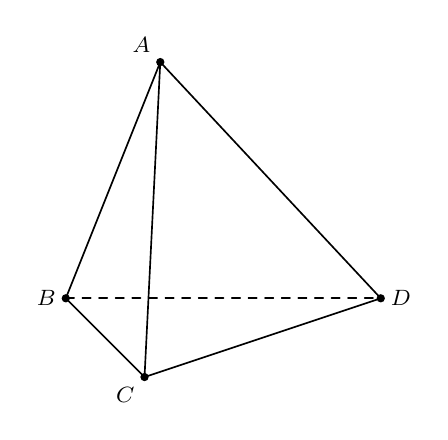
\begin{tikzpicture}[line join=round,line cap=round,line width=.6pt,font=\footnotesize,scale=1]
				\coordinate[label=left:$B$] (B) at (0,0);
				\coordinate[label=below left:$C$] (C) at (1,-1);
				\coordinate[label=right:$D$] (D) at (4,0);
				\coordinate[label=above left:$A$] (A) at (1.2,3);
				\draw (B)--(C)--(D)--(A)--cycle (A)--(C);
				\draw[dashed] (B)--(D);
				\fill (B)circle(1.5pt) (C)circle(1.5pt) (D)circle(1.5pt) (A)circle(1.5pt);
			\end{tikzpicture}
		}
	}		
\end{vd}
%% Ví dụ 3
\begin{vd}%[2H2H1-2]%[Dự án đề cương 3 khối NH24-25-Dot1-Nguyen Huynh]
	Cho hình hộp $ABCD.A'B'C'D'$. Gọi $G$ là trọng tâm tam giác $AB'D'$. Chứng minh rằng $\overrightarrow{A'C}=3 \overrightarrow{A'G}$.
	\loigiai{
		\immini{Theo quy tắc hình hộp, ta có: 	$\overrightarrow{A'A}+\overrightarrow{A'B'}+\overrightarrow{A'D'}=\overrightarrow{A'C}$.\\
			Mặt khác, áp dụng tính chất trọng tâm trong $\triangle AB'D'$, ta được:
			$$\overrightarrow{A'A}+\overrightarrow{A'B'}+\overrightarrow{A'D'}=3 \overrightarrow{A'G}.$$
			Do đó, $\overrightarrow{A'C}=3 \overrightarrow{A'G}$.
		}
		{\begin{tikzpicture}[line join=round,line cap=round,line width=.6pt,font=\footnotesize,scale=0.6]
				\coordinate[label=below left:$B$] (B) at (0,0);
				\coordinate[label=left:$A$] (A) at (1,.8);
				\coordinate[label=below right:$C$] (C) at (3,0);
				\coordinate[label=right:$D$] (D) at ($(C)-(B)+(A)$);
				\coordinate (H) at ($(B)!1/3!(D)$);
				\coordinate[label=left:$A'$] (A1) at ($(H)+(110:4)$);
				\coordinate[label=left:$B'$] (B1) at ($(B)-(A)+(A1)$);
				\coordinate[label=below left:$C'$] (C1) at ($(C)-(A)+(A1)$);
				\coordinate[label=right:$D'$] (D1) at ($(D)-(A)+(A1)$);
				\draw (B1)--(B)--(C)--(D)--(D1)--(A1)--(B1)--(C1)--(D1) (C)--(C1) (B1)--(D1);
				%\draw[-{Stealth[length=2mm]}] (D1)--(A)--(A1);
				\draw[dashed] (C)--(A)--(D) (A1)--(A)--(B) (D1)--(A)--(B1);
				\fill (A)circle(1.5pt) (B)circle(1.5pt) (C)circle(1.5pt) (D)circle(1.5pt) (A1)circle(1.5pt) (B1)circle(1.5pt) (C1)circle(1.5pt) (D1)circle(1.5pt);
			\end{tikzpicture}
		}
	}		
\end{vd}
%%%=============BT_5=============%%%
\begin{vd}%[2H2H1-2]%[Dự án đề cương 3 khối NH24-25-Dot1-Nguyen Huynh]
	Cho hình lập phương $ABCD.A'B'C'D'$. Gọi $O$, $O'$ lần lượt là tâm của các hình vuông $ABCD$ và $A'B'C'D'$; $I$ là giao điểm của $AC'$ và $A'C$. Chứng minh rằng
	\begin{multicols}{2}
		\begin{enumerate}
			\item $\overrightarrow{OA'}+\overrightarrow{OB'}+\overrightarrow{OC'}+\overrightarrow{OD'}=4\overrightarrow{OO'}$;
			\item $\overrightarrow{DB}+\overrightarrow{DD'}=2\overrightarrow{DI}$.
		\end{enumerate}
	\end{multicols}
	\loigiai{
		\immini{
			\begin{enumerate}
				\item $\overrightarrow{OA'}+\overrightarrow{OB'}+\overrightarrow{OC'}+\overrightarrow{OD'}=(\overrightarrow{OA'}+\overrightarrow{OC'})+(\overrightarrow{OB'}+\overrightarrow{OD'})$ $$=2 \overrightarrow{OO'}+2 \overrightarrow{OO'}=4 \overrightarrow{OO'}
				$$
				\item Ta có bốn đường chéo của hình lập phương cắt nhau tại trung điểm $I$ của mỗi đường nên $I$ cũng là trung điểm của $DB'$.\\
				Suy ra $\overrightarrow{DB}+\overrightarrow{DD'}=\overrightarrow{DB'}=2\overrightarrow{DI}$.
			\end{enumerate}
		}{
			\begin{tikzpicture}[scale=0.6, font=\footnotesize,line join=round, line cap=round, >=stealth]
				\path 
				(0,0) coordinate (A)
				++(-130:3) coordinate (B)
				++(0:4) coordinate (C)
				($(A)+(C)-(B)$) coordinate (D)
				($(A)!1/2!(C)$) coordinate (O)
				;
				\foreach \i in {A,B,C,D}{
					\coordinate (\i') at ($(\i)+(0,4)$);
				}
				\path ($(A')!1/2!(C')$) coordinate (O')
				($(O)!1/2!(O')$) coordinate (I);
				\draw (A')--(B')--(C')--(D')--cycle;
				\draw (B)--(B') (C)--(C') (D)--(D')  (B)--(C)--(D) (A')--(C');
				\draw[dashed,thin](B)--(A)--(A') (C)--(A)--(D)--(B)
				(D)--(B') (A)--(C') (C)--(A') (O)--(O')
				;	
				\foreach \i/\g in {A'/180,B'/180,C'/0,D'/0,A/180,B/-90,C/-90,D/0,O/-90,O'/80,I/-40}
				\fill[black] (\i) circle(1pt)+(\g:0.4)node[scale=1]{$\i$};
			\end{tikzpicture}
		}				
	}
\end{vd}
\begin{dang}{Ứng dụng của tích vô hướng}
\end{dang}
\setcounter{vd}{0}
\begin{vd}%[2H2H1-3]%[Dự án đề cương 3 khối NH24-25-Dot1-Nguyen Huynh]
	Cho hình lập phương $ABCD.A'B'C'D'$ có cạnh bằng $a$. Tính:
	\begin{listEX}[2]
		\item $\overrightarrow{A'B} \cdot \overrightarrow{D'C}$; $\overrightarrow{D'A} \cdot \overrightarrow{BC}$;
		\item Các góc $\left(\overrightarrow{A'D}, \overrightarrow{B'C'}\right);\left(\overrightarrow{AD'}, \overrightarrow{BD}\right)$.
	\end{listEX}
	\loigiai{
		\immini{\begin{enumerate}[a)]
				\item Sử dụng định nghĩa tích vô hướng của hai vectơ trong không gian, ta có:
				\allowdisplaybreaks
				\begin{eqnarray*}
					\overrightarrow{A'B} \cdot \overrightarrow{D'C'}
					&=& \left|\overrightarrow{A'B}\right| \cdot\left|\overrightarrow{D'C}\right| \cdot \cos \left(\overrightarrow{A'B'}, \overrightarrow{D'C'}\right)\\
					&=& a \sqrt{2} \cdot a \cdot \cos \left(\overrightarrow{A'B}, \overrightarrow{A'B}\right)=a^2 \sqrt{2} \cdot \cos 45^\circ=a^2.
				\end{eqnarray*}
				\begin{eqnarray*}
					\overrightarrow{D'A} \cdot \overrightarrow{BC}
					&=& -\overrightarrow{AD'} \cdot \overrightarrow{BC}\\
					&=& -\left|\overrightarrow{AD'}\right| \cdot\left|\overrightarrow{BC}\right| \cdot \cos \left(\overrightarrow{AD'}, \overrightarrow{B C}\right)\\
					&=&-a \sqrt{2} \cdot a \cdot \cos(\overrightarrow{AD'}, \overrightarrow{AD})=-a^2 \sqrt{2} \cdot \cos 45^\circ=-a^2.
				\end{eqnarray*}
				\item Ta có $\left(\overrightarrow{A'D}, \overrightarrow{B'C'}\right)=\left(\overrightarrow{A'D}, \overrightarrow{A' D'}\right)=45^\circ$;\\
				Với $(\overrightarrow{AD}, \overrightarrow{BD})=(\overrightarrow{BC}, \overrightarrow{BD})=\widehat{C'BD}$ mà $\triangle C'BD$ đều nên $\widehat{C'BD}=60^\circ$.\\
				Vậy $\left(\overrightarrow{AD'}, \overrightarrow{B D}\right)=60^\circ$.
			\end{enumerate}
		}
		{\begin{tikzpicture}[scale=0.6, font=\footnotesize, line join=round, line cap=round, >=stealth]
				\def\bc{4} \def\ba{2} \def\h{4} \def\gocB{35} 
				\coordinate[label=below left:$B$] (B) at (0,0);
				\coordinate[label=above left:$A$] (A) at (\gocB:\ba);
				\coordinate[label=below:$C$] (C) at (\bc,0);
				\coordinate[label=right:$D$] (D) at ($(C)-(B)+(A)$);
				\coordinate[label=above left:$A'$] (A') at ($(A)+(90:\h)$);
				\coordinate[label=left:$B'$] (B') at ($(B)-(A)+(A')$);
				\coordinate[label=above left:$C'$] (C') at ($(C)-(A)+(A')$);
				\coordinate[label=right:$D'$] (D') at ($(D)-(A)+(A')$);
				\draw (B')--(B)--(C)--(D)--(D')--(A')--(B')--(C')--(D') (C)--(C') (B')--(C);
				\draw[dashed] (A')--(A)--(D) (A)--(B);
				\draw[-{Stealth[length=2mm]},dashed] (A')--(B);
				\draw[-{Stealth[length=2mm]}] (D')--(C);
				\draw[-{Stealth[length=2mm]},dashed] (D')--(A);
				\foreach \diem in {A,B,C,D,A',B',C',D'}	\fill (\diem)circle(1pt);
			\end{tikzpicture}
		}
	}		
\end{vd}
%%%=============BT_6=============%%%
\begin{vd}%[2H2H1-3]%[Dự án đề cương 3 khối NH24-25-Dot1-Nguyen Huynh]
	Cho hình hộp $ABCD.A'B'C'D'$ có tất cả các cạnh bằng $a$ và cho biết \break  $\widehat{BAD}=\widehat{BAA'}=\widehat{DAA'}=60^\circ$. Tính các tích vô hướng sau:
	\begin{multicols}{3}
		\begin{enumerate}
			\item $\overrightarrow{AB}\cdot \overrightarrow{AD}$;
			\item $\overrightarrow{DA}\cdot \overrightarrow{DC}$;
			\item $\overrightarrow{AA'}\cdot \overrightarrow{AC}$.
		\end{enumerate}
	\end{multicols}
	\loigiai{
		\begin{center}
			\begin{tikzpicture}[scale=0.6, font=\footnotesize,line join=round, line cap=round, >=stealth]
				\path 
				(0,0) coordinate (A)
				++(-130:3) coordinate (B)
				++(0:4) coordinate (C)
				($(A)+(C)-(B)$) coordinate (D)
				($(A)!1/2!(C)$) coordinate (O)
				;
				\foreach \i in {A,B,C,D}{
					\coordinate (\i') at ($(\i)+(0.5,4)$);
				}
				\draw (A')--(B')--(C')--(D')--cycle;
				\draw (B)--(B') (C)--(C') (D)--(D')  (B)--(C)--(D) (A')--(C');
				\draw[dashed,thin](B)--(A)--(A') (C)--(A)--(D);	
				\foreach \i/\g in {A'/90,B'/90,C'/90,D'/90,A/-90,B/-90,C/-90,D/-90}
				\fill[black] (\i) circle(1pt)+(\g:5mm)node[scale=1]{$\i$};
			\end{tikzpicture}
		\end{center}
		\begin{enumerate}
			\item 
			\begin{align*}
				\overrightarrow{AB}\cdot \overrightarrow{AD}&=\left|\overrightarrow{AB}\right| \cdot\left|\overrightarrow{AD}\right|\cdot \cos \Big(\overrightarrow{AB},\overrightarrow{AD}\Big)\\
				&=AB\cdot AD\cdot \cos \widehat{BAD}=a\cdot a\cdot \cos 60^\circ=\dfrac{a^2}{2}.
			\end{align*}
			\item
			\begin{align*}
				\overrightarrow{DA}\cdot \overrightarrow{DC}&=\left|\overrightarrow{DA}\right| \cdot\left|\overrightarrow{DC}\right|\cdot \cos \Big(\overrightarrow{DA},\overrightarrow{DC}\Big)\\
				&=DA\cdot DC\cdot \cos \widehat{ADC}=a \cdot a \cdot \cos 120^\circ=-\dfrac{a^2}{2}.
			\end{align*}
			\item 
			\begin{align*}
				\overrightarrow{AA'}\cdot \overrightarrow{AC}&=\overrightarrow{AA'} \cdot \Big(\overrightarrow{AB}+\overrightarrow{AD}\Big)\\
				&=\overrightarrow{AA'}\cdot \overrightarrow{AB}+\overrightarrow{AA'}\cdot \overrightarrow{AD} =\dfrac{a^2}{2}+\dfrac{a^2}{2}=a^2.
			\end{align*}
		\end{enumerate}	
	}
\end{vd}
\begin{vd}%[2H2H1-3]%[Dự án đề cương 3 khối NH24-25-Dot1-Nguyen Huynh]
	Trong không gian, cho hai vectơ $\overrightarrow{a}$ và $\overrightarrow{b}$ cùng có độ dài bằng $1$. Biết rằng góc giữa hai vectơ đó là $45^{\circ}$, hãy tính
	\begin{enumerate}[a)]	
		\item  $\overrightarrow{a}\cdot \overrightarrow{b}$;
		\item  $\left( \overrightarrow{a}+3 \overrightarrow{b}\right)  \cdot\left( \overrightarrow{a}-2 \overrightarrow{b}\right) $;
		\item  $\left( \overrightarrow{a}+ \overrightarrow{b}\right)^2 $.
	\end{enumerate}
	\loigiai{Ta có  $\left| \overrightarrow{a}\right| =\left| \overrightarrow{b}\right| =1$, $\left(\overrightarrow{a},\overrightarrow{b} \right) =45^\circ$. 
		\begin{enumerate}[a)]	
			\item  $\overrightarrow{a}\cdot \overrightarrow{b}=\left| \overrightarrow{a}\right|\cdot \left| \overrightarrow{b}\right|\cos \left(\overrightarrow{a},\overrightarrow{b} \right)=\dfrac{\sqrt{2}}{2}$.
			\item  $\left( \overrightarrow{a}+3 \overrightarrow{b}\right)  \cdot\left( \overrightarrow{a}-2 \overrightarrow{b}\right)=\left| \overrightarrow{a}\right|^2+\cdot\overrightarrow{a}\cdot \overrightarrow{b}-6\left| \overrightarrow{b}\right|^2 =1+\cdot\dfrac{\sqrt{2}}{2}-6=-5+\dfrac{\sqrt{2}}{2} $.
			\item  $\left( \overrightarrow{a}+ \overrightarrow{b}\right)^2= \overrightarrow{a}^2+2\overrightarrow{a}\cdot \overrightarrow{b}+\overrightarrow{b}^2=1+2\cdot\dfrac{\sqrt{2}}{2}+1=2+\sqrt{2}$.
		\end{enumerate}		
	}
\end{vd}
\begin{dang}{Ứng dụng}
\end{dang}
%% Ví dụ 5
%%%=============BT_7=============%%%
\begin{vd}%[2H2V1-3]%[Dự án đề cương 3 khối NH24-25-Dot1-Nguyen Huynh]
	\immini{
		Một tàu kéo một xà lan trên biển di chuyển được $3$ km với một lực kéo có cường độ $2\,000$ N và có phương hợp với phương dịch chuyển một góc $30^\circ$. Tính công thực hiện bởi lực kéo nói trên (kết quả làm tròn đến hàng đơn vị của Jun).
	}{
		\begin{tikzpicture}[scale=0.7, font=\footnotesize,line join=round, line cap=round, >=stealth]
			\draw[->] (0,0)--(8,0)node[scale=1,shift=(-140:0.6)]{$\overrightarrow {d}$};
			\draw [fill=black,opacity=0.4] (0.2,0) rectangle  (2,0.3);
			\draw[->] (2,0)--++(30:4)node[opacity=0.8,scale=4,shift=(-90:0.19)]{\faShip};
			\path (2,0.3)node[scale=1,shift=(0:0.8)]{$30^\circ$}
			(3,1.2)node[scale=1,shift=(0:0.1)]{$\overrightarrow {F}$};	
		\end{tikzpicture}
	}
	\loigiai{
		Áp dụng công thức tính công, ta có\\
		$A=\overrightarrow{F}\cdot \overrightarrow{d}=\left|\overrightarrow{F}\right| \cdot\left|\overrightarrow{d}\right|\cdot \cos \Big(\overrightarrow{F}, \overrightarrow{d}\Big)=2\,000\cdot 3\,000\cdot \cos 30^\circ\approx 5\,196\,152$ (J).
	}
\end{vd}
%%%=============BT_3=============%%%
\begin{vd}%[2H2V1-4]%[Dự án đề cương 3 khối NH24-25-Dot1-Nguyen Huynh]
	Có ba lực cùng tác động vào một vật. Hai trong ba lực này hợp với nhau một góc $120^\circ$ và có độ lớn lần lượt là $10$ N và $8$ N. Lực thứ ba vuông góc với mặt phẳng tạo bởi hai lực đã cho và có độ lớn $6$ N. Tính độ lớn của hợp lực của ba lực trên.
	\loigiai{
		\immini{
			Gọi $\overrightarrow{F}_1$, $\overrightarrow{F}_2$, $\overrightarrow{F}_3$ lần lượt là ba lực tác động vào một vật đặt tại điểm $O$ như hình.\\ 
			Ta có $\overrightarrow{F}_1=\overrightarrow{OA}$, $\overrightarrow{F}_2=\overrightarrow{OB}$, $\overrightarrow{F}_3=\overrightarrow{OC}$.\\
			Độ lớn các lực\\ 
			$F_1=OA=10$ N, $F_2=OB=8$ N, $F_3=OC=6$ N.\\
			Dựng hình bình hành $OADB$, $ODEC$.	
		}{ 
			\begin{tikzpicture}[scale=1.6, font=\footnotesize, line join=round, line cap=round,>=stealth]
				\foreach \x\y\t in {0/0/O,2/0/A,-0.5/-0.9/B,0/1.5/C}
				\coordinate (\t) at (\x,\y);
				\coordinate (D) at ($(A)+(B)$);
				\coordinate (E) at ($(C)+(D)$);
				\foreach \a\b in {O/A,O/B,O/C,O/D,O/E}
				\draw[->] (\a)--(\b);
				\path 
				(O)--(A) node[pos=0.85,above]{$\overrightarrow{F_1}$}
				(O)--(B) node[pos=0.7,left]{$\overrightarrow{F_2}$}
				(O)--(C) node[pos=0.5,above left]{$\overrightarrow{F_3}$};
				\path 
				(O) node[scale=1,shift=(-70:.4)]{$120^\circ$}
				pic[draw,angle radius=8]{angle=B--O--A}
				pic[draw,angle radius=4]{right angle=C--O--B}
				pic[draw,angle radius=4]{right angle=C--O--A};
				\foreach \t\g in {A/90, B/-90, C/180,D/-90,E/0,O/180}
				\draw[fill=black] (\t)circle(0.1pt) +(\g:0.15)node[scale=1]{$\t$};
				\draw[dashed] (B)--(D)--(A) (D)--(E)--(C);
			\end{tikzpicture}
		}\noindent
		Theo quy tắc hình bình hành, ta có $\overrightarrow{OD}=\overrightarrow{OA}+\overrightarrow{OB}$.\\
		Suy ra ${\overrightarrow{OD}}^2=\Big(\overrightarrow{OA}+\overrightarrow{OB}\Big)^2={\overrightarrow{OA}}^2+{\overrightarrow{OB}}^2+2\overrightarrow{OA}\cdot \overrightarrow{OB}$.\\
		Mà $\overrightarrow{OA}\cdot \overrightarrow{OB}=OA\cdot OB\cdot \cos (\overrightarrow{OA},\overrightarrow{OB})$.\\
		Suy ra $OD^2=OA^2+OB^2+2\cdot OA\cdot OB\cdot \cos 120^\circ$.\\
		Tổng lực tác động vào vật là $\overrightarrow{F}=\overrightarrow{OE}=\overrightarrow{OA}+\overrightarrow{OB}+\overrightarrow{OC}$.\\
		Độ lớn của hợp lực tác động vào vật là $F=OE$.\\
		Vì $OC\perp(OADB)$ nên $OC\perp OD$, suy ra $ODEC$ là hình chữ nhật.\\
		Do đó tam giác $ODE$ vuông tại $D$.\\
		Khi đó $OE^2=OC^2+OD^2=OC^2+OA^2+OB^2+2\cdot OA\cdot OB\cdot \cos 120^\circ$.\\
		Suy ra 
		\begin{align*}
			OE&=\sqrt{OC^2+OA^2+OB^2+2\cdot OA\cdot OB\cdot \cos 120^\circ}\\
			&=\sqrt{6^2+10^2+8^2+2\cdot 10\cdot 8\cdot \cos 120^\circ}\approx 10{,}95.
		\end{align*}
		Do đó $F=OE\approx 10{,}95$ (N).
	}
\end{vd}
\begin{vd}%[2H2V1-4]%[Dự án đề cương 3 khối NH24-25-Dot1-Nguyen Huynh]
	\immini
	{Một chiếc ô tô được đặt trên mặt đáy dưới của một khung sắt có dạng hình hộp chữ nhật với đáy trên là hình chữ nhật $ABCD$, mặt phẳng $(ABCD)$ song song với mặt phẳng nằm ngang. Khung sắt đó được buộc vào móc $E$ của chiếc cần cẩu sao cho các doạn dây cáp $EA$, $EB$, $EC$, $ED$ có độ dài bằng nhau và cùng tạo với mặt phẳng $(ABCD)$ một góc bằng $60^{\circ}$. Chiếc cần cẩu kéo khung sắt lên theo phương thằng đứng. Tỉnh trọng lượng của chiếc xe ô tô (làm tròn kết quả đến hàng đơn vị). Biết rằng các lực căng $\overrightarrow{F_1}$, $\overrightarrow{F_2}$, $\overrightarrow{F_3}$, $\overrightarrow{F_4}$ đều có cường độ là $4\,700$ N và trọng lượng của khung sắt là $3\,000$ N.
	}
	{\begin{tikzpicture}[>=latex,line join=round, line cap=round,scale=0.65,transform shape]
			\definecolor{bostonuniversityred}{rgb}{0.8, 0.0, 0.0}
			\definecolor{charcoal}{rgb}{0.21, 0.27, 0.31}
			\definecolor{bananayellow}{rgb}{1.0, 0.88, 0.21}
			\definecolor{anti-flashwhite}{rgb}{0.95, 0.95, 0.96}
			%	\clip (-6,-3) rectangle (6,3);
			\tikzset{%
				xeoto/.pic={%
					%--------------------------	
					\tikzset{xe/.pic={
							\def\N{ 
								(-2.7,.56)--(-2.5,.56)
								..controls +(50:1.5) and +(165:1.5) .. (2.1,1.88)--(2.05,2)
								..controls +(-10:.1) and +(130:.1) .. (3.25,1.75)--(3.15,1.65)
								..controls +(-4:.2) and +(130:.15) .. (4.05,.7)--(4.25,.75)
								..controls +(-40:.2) and +(130:.15) .. (4.55,.35)--(4.35,.26)
								..controls +(-40:.2) and +(130:.15) .. (4.8,-.45)--(4.92,-.4)
								..controls +(-40:.25) and +(73:.17) .. (4.8,-1.8)--(-4.4,-1.8)
								..controls +(175:.7) and +(-175:3.2) ..cycle
								;
							}
							\fill[bostonuniversityred] \N;
							\draw \N;
							\def\K{ 
								(-2.2,.56)--(3.3,.7)
								..controls +(100:1.18) and +(43:3) .. cycle
								;
							}
							\fill[bottom color=charcoal,top color=charcoal!20!white, middle color=charcoal!80!white] \K;
							\draw \K;
							\def\K1{ 
								(-2.2,.56)
								..controls +(43:.2) and +(43:.2) .. (-1.58,1.05)--(-1.53,.57)--cycle
								;
							}
							\draw \K1;
							\fill[charcoal] \K1;
							\def\K2{ 
								(1.2,1.85)
								..controls +(-10:.1) and +(160:.1) .. (1.58,1.8)--(1.8,.65)--(1.25,.65)--cycle
								;
							}
							\draw \K2;
							\fill[charcoal] \K2;
							\def\Kt{ 
								(-2.5,.56)
								..controls +(50:1.5) and +(165:1.5) .. (2.1,1.88)--(2.05,2)
								..controls +(170:2.2) and +(45:1.5) .. (-2.7,.56)--cycle
								;
							}
							\fill[charcoal!50] \Kt;
							\draw \Kt;
							\def\Ks{ 
								(3.25,1.75)--(3.15,1.65)
								..controls +(-4:.2) and +(130:.15) .. (4.05,.7)--(4.22,.75)
								..controls +(120:.3) and +(-35:.3) .. cycle
								;
							}
							\fill[charcoal!50] \Ks;
							\draw \Ks;
							%Đèn sau
							\def\D{ 
								(4.55,.35)--(4.35,.26)
								..controls +(-40:.2) and +(130:.15) .. (4.8,-.45)--(4.92,-.4)
								..controls +(110:.2) and +(-40:.15) ..cycle
								;
							}
							\fill[bananayellow] \D;
							\draw \D;
							\def\M{ 
								(2.2,-1.3)--(-1.8,-1.4)--(-1.78,-1.7)
								..controls +(-5:.3) and +(-90:.6) ..cycle
								;
							}
							\draw \M;
							\fill[charcoal!90] \M;
							\draw (-1.6,.55)
							..controls +(-170:.5) and +(95:.4) .. (-1.78,-1.7)
							(1.6,.65)
							..controls +(-30:.5) and +(35:.3) .. (1.7,-1.3)
							;
							%gương
							\def\G{ 
								(-1.5,.45)--(-1.4,.6)
								..controls +(85:1) and +(20:.6) .. (-1.25,.5)--(-1.4,.33)
								;
							}
							\draw \G;
							\fill[bostonuniversityred] \G;
							%Đèn trước
							\def\Dt{ 
								(-4.85,-.7)
								..controls +(75:1) and +(65:.8) .. (-4.5,-.7)
								..controls +(-115:.6) and +(-105:.4) .. cycle
								;
							}
							\fill[bananayellow] \Dt;
							\draw \Dt;
							\def\Dt2{ 
								(-4.85,-.7)
								..controls +(75:.6) and +(65:.4) .. (-4.7,-.7)
								..controls +(-115:.3) and +(-105:.2) .. cycle
								;
							}
							\fill[anti-flashwhite] \Dt2;
							\draw \Dt2;
							\draw[fill=anti-flashwhite] (-4.86,-1.45)--(-4.82,-1.5)--(-4.55,-1.3)
							..controls +(90:.3) and +(45:.2) .. cycle;
					}}
					\tikzset{banh_xe/.pic={
							\draw[fill=charcoal] (-3.25,-1.65) circle (1) ;
							\draw[fill=anti-flashwhite] (-3.25,-1.65) circle (.7) ;
							\draw[fill=charcoal] (-3.25,-1.65) circle (.4) ;
					}}
					%----------------
					\path
					(0,0)pic[scale=1]{xe}(0,0)pic[scale=1]{banh_xe}(6.9,0)pic[scale=1]{banh_xe};
					%--------------------------------
			}}
			%%%%%%%%%%%%%%%%%%%
			\def\bc{4.25} % cạnh BC
			\def\ba{1.5} % cạnh BA
			\def\h{4} % đường cao
			\def\gocnghieng{90} % góc nghiêng
			\def\gocB{160} % góc B của đáy
			\coordinate (B1) at (0,0);
			\coordinate (A1) at (\gocB:\ba);
			\coordinate (C1) at (\bc,0.25);
			\coordinate (D1) at ($(C1)-(B1)+(A1)$);
			\coordinate[label=above left:$A$] (A) at ($(A1)+(\gocnghieng:\h)$);
			\coordinate[label=below left:$B$] (B) at ($(B1)-(A1)+(A)$);
			\coordinate[label=right:$C$] (C) at ($(C1)-(A1)+(A)$);
			\coordinate[label=above right:$D$] (D) at ($(D1)-(A1)+(A)$);
			\coordinate (E) at ($(A)!0.5!(C)+(\gocnghieng:\h)$);
			\coordinate (O) at ($(A)!0.5!(C)$);
			\path (O) node[below]{$O$};
			%------------
			%\draw[->,blue,very thick] (E)--($(E)!0.5!(A)$) ;
			%\draw[->,blue,very thick] (E)--($(E)!0.5!(B)$) ;
			\draw[->,blue,very thick] (E)--($(E)!0.5!(C)$) node[above right]{$\overrightarrow{F3}$};
			\draw[->,blue,very thick] (E)--($(E)!0.5!(D)$) node[below left]{$\overrightarrow{F4}$};
			\draw[->,blue,very thick] (E)--($(E)!0.5!(A)$) node[above left]{$\overrightarrow{F1}$};
			\draw[->,blue,very thick] (E)--($(E)!0.5!(B)$) node[below right]{$\overrightarrow{F2}$};
			%\draw[->,blue,very thick] (E)--($(E)!0.4!(D)$) ;
			\draw[dashed] (A)--(C) (B)--(D);
			\draw[dashed] (E)--(O);
			%------------
			\path (E) node[left=1mm]{$E$};
			\draw[blue,very thick] (A)--(B)--(C)--(D)--cycle
			(A1)--(A) (D1)--(D) (C1)--(C)
			(A)--(E)--(B) (C)--(E)--(D);
			\draw[fill=teal] (A1)--(B1)--(C1)--(D1)--cycle;
			\draw[fill=teal!30] (A1)--(B1)--(C1)--++(0,-0.3)--([yshift=-0.3cm]B1)--([yshift=-0.3cm]A1)--cycle;
			\foreach \diem in {A1,B1,C1,D1,A,B,C,D,E}	\fill (\diem)circle(1.5pt);
			%phần móc và dây
			\def\r{0.3}\def\rr{0.25}
			\coordinate (tam) at ([yshift=6mm]E);
			\draw[brown,fill=brown,line width=1pt] (tam) circle (\r cm);
			\fill (tam) circle (2pt);
			\draw[brown,line width=1pt] (tam)++(\r,0)--++(0,0.7)
			(tam)++(-\r,0)--++(0,0.7);
			\draw[line width=1.5pt] (tam)--++(0,-1.35*\r) arc(90:370:1mm);
			%%%%%%%%%%%%%%%%%%%
			\pic[scale=0.45,rotate=4] at (1.6,1.3) [pic type = xeoto];
			%--------
			\draw[blue,very thick] (B)--(B1);		
		\end{tikzpicture}
	}
	\loigiai{
		\immini{Gọi $A_1$, $B_1$, $C_1$, $D_1$ lần lượt là các diểm sao cho
			$$\overrightarrow{EA_1}=\overrightarrow{F_1}, \overrightarrow{EB_1}=\overrightarrow{F_2}, \overrightarrow{EC_1}=\overrightarrow{F_3}, \overrightarrow{ED_1}=\overrightarrow{F_4}.$$
			Do các lực căng $\overrightarrow{F}_1, \overrightarrow{F}_2, \overrightarrow{F}_3, \overrightarrow{F}_4$ đều có cường độ là $4\,700$ N nên $$\left|\overrightarrow{F}_1\right|=\left|\overrightarrow{F}_2\right|=\left|\overrightarrow{F}_3\right|=\left|\overrightarrow{F}_3\right|=4\,700 N.$$ 
			Gọi $O$ là tâm của hình chữ nhật $A_1B_1C_1D_1$.\\
			Khi đó, $O$ là trung điểm của $A_1 C_1$ và $B_1 D_1$.\\
			Sử dụng quy tắc trung diểm ta có: $\heva{&\overrightarrow{F_1}+\overrightarrow{F_3}=2 \overrightarrow{EO}\\&\overrightarrow{F_2}+\overrightarrow{F_4}=2 \overrightarrow{EO}.}$\\
			Suy ra, $\overrightarrow{F_1}+\overrightarrow{F_2}+\overrightarrow{F_3}+\overrightarrow{F_4}=4 \overrightarrow{EO}$.		
		}
		{\begin{tikzpicture}[line join=round,line cap=round,line width=.6pt,font=\footnotesize,scale=1]
				\coordinate[label=below left:$B1$] (B) at (0,0);
				\coordinate[label=above right:$A1$] (A) at (1,.8);
				\coordinate[label=below right:$C1$] (C) at (4,0);
				\coordinate[label=above right:$D1$] (D) at ($(C)-(B)+(A)$);
				\coordinate[label=below:$O$] (O) at ($(A)!.5!(C)$);
				\coordinate[label=above left:$S$] (S) at ($(O)+(90:4)$);
				\draw (B)--(C)--(D)--(S)--cycle (S)--(C);
				\draw[dashed] (C)--(A)--(D)--(B) (O)--(S)--(A)--(B);
				\fill (A)circle(1.5pt) (B)circle(1.5pt) (C)circle(1.5pt) (D)circle(1.5pt) (S)circle(1.5pt) (O)circle(1.5pt);
			\end{tikzpicture}
		}\noindent
		Mặt khác, do các cạnh $EA$, $EB$, $EC$, $ED$ tạo với với mặt phẳng $(ABCD)$ một góc bằng $60^{\circ}$ nên 
		$$\widehat{EA_1O}=\widehat{EB_1O}=\widehat{EC_1O}=\widehat{ED_1O}=60^{\circ}.$$
		Do đó $\triangle EA_1C_1$ là tam giác đều cạnh $4\,700$ N với dường cao $EO=2\,350 \sqrt{3}$ N.\\
		Do khung sắt ở vị tri cân bằng nên $\overrightarrow{F_1}+\overrightarrow{F_2}+\overrightarrow{F_3}+\overrightarrow{F_4}=\overrightarrow{P}$, ở đó $\overrightarrow{P}$ là trọng lực tác dụng lên chiếc xe ô tô và khung sắt. Ta tính được tổng trọng lực có độ lớn là $4|\overrightarrow{O E}|=9\,400 \sqrt{3}$ N.\\
		Vậy trọng lực của ô tô bằng $9\,400 \sqrt{3}-3\,000 \approx 13\,281$ N.
	}	
\end{vd}


%-----------------------------------------------------------------------------
\subsection{Bài tập rèn luyện}
\ind{PHẦN I.} \inden{Câu trắc nghiệm nhiều phương án lựa chọn. Mỗi câu hỏi học sinh chỉ chọn một phương án.}\\
\setcounter{ex}{0}
\Opensolutionfile{ans}[ans/2H2-Bai1-TN]%--Đặt tên 2D1-Bai1-Dang1-TN
\begin{ex}%[2H2N1-2]%[Dự án đề cương 3 khối NH24-25-Dot1-Nguyen Huynh]
	Trong không gian cho $3$ điểm $M$, $N$, $P$ phân biệt. Tính $\overrightarrow{PM}+\overrightarrow{MN}$.
	\choice
	{$\overrightarrow{NM}$}
	{$\overrightarrow{MN}$}
	{$\overrightarrow{NP}$}
	{\True $\overrightarrow{PN}$}
	\loigiai{Theo quy tắc ba điểm ta có $\overrightarrow{PM}+\overrightarrow{MN}=\overrightarrow{PN}$.
	}
\end{ex}


\begin{ex}%[2H2H1-2]%[Dự án đề cương 3 khối NH24-25-Dot1-Nguyen Huynh]
	\immini{
		Cho hình lập phương $ABCD.A'B'C'D'$. Vectơ có điểm đầu và điểm cuối là các đỉnh của hình lập phương $ABCD.A'B'C'D'$ và bằng vectơ $\overrightarrow{AD}$ là
		\choice
		{\True $\overrightarrow{B'C'}$}
		{$\overrightarrow{DA}$}
		{$\overrightarrow{CB}$}
		{$\overrightarrow{AB}$}
	}{
		\begin{tikzpicture}[scale=0.8,font=\footnotesize,line join=round,line cap=round,>=stealth]
			\def\a{3.5}
			\path (0:0) coordinate (A)
			++(0:\a) coordinate (D)
			++(-130:\a/2) coordinate (C)
			($(A)+(C)-(D)$) coordinate (B)
			($(A)+(90:\a)$) coordinate (A')
			($(B)+(90:\a)$) coordinate (B')
			($(C)+(90:\a)$) coordinate (C')
			($(D)+(90:\a)$) coordinate (D');
			\draw[dashed] (B)--(A)--(D) (A)--(A');
			\draw (C)--(C') (D)--(D') (B)--(B') (B)--(C)--(D) (A')--(B')--(C')--(D')--cycle;
			\foreach \x/\g in {A/180,B/180,C/0,D/0,A'/180,B'/180,C'/0,D'/0}
			\fill (\x) circle (1pt)
			($(\g:4mm)+(\x)$) node {$\x$}; 
		\end{tikzpicture}
	}
	\loigiai{Do $ABCD.A'B'C'D'$ là hình lập phương nên ta có $AD=B'C'$.\\
		Ta thấy $\overrightarrow{AD}$ và $\overrightarrow{B'C'}$ cùng hướng.\\
		Do đó $\overrightarrow{AD}=\overrightarrow{B'C'}$.
	}
\end{ex}


\begin{ex}%[2H2H1-2]%[Dự án đề cương 3 khối NH24-25-Dot1-Nguyen Huynh]
	Gọi $I$ là trung điểm của $AB$, $M$ là điểm bất kì. Khẳng định nào sau đây \textbf{sai}?
	\choice
	{$\overrightarrow{IA}+\overrightarrow{IB}=\overrightarrow{0}$}
	{$IA=IB$}
	{\True $\overrightarrow{IA}=\overrightarrow{IB}$}
	{$\overrightarrow{MA}+\overrightarrow{MB}=2\overrightarrow{MI}$}
	\loigiai{
		\begin{center}
			\begin{tikzpicture}[scale=1,font=\footnotesize,line join=round,line cap=round,>=stealth]
				\path (0:0) coordinate (A)
				(0:4) coordinate (B)
				($(A)!0.5!(B)$) coordinate (I);
				\draw[->] (I)--(A);
				\draw[->] (I)--(B);
				\foreach \x/\g in {A/90,B/90}
				\fill ($(\g:4mm)+(\x)$) node {$\x$}; 
				\foreach \x/\g in {I/90}
				\fill (\x) circle (1pt)
				($(\g:4mm)+(\x)$) node {$\x$}; 
			\end{tikzpicture}
		\end{center} 
		$I$ là trung điểm của $AB$ nên ta có $IA=IB$ và hai vectơ $\overrightarrow{IA}$, $\overrightarrow{IB}$ ngược hướng. Do đó $\overrightarrow{IA}=-\overrightarrow{IB}$.\\
		Vậy khẳng định sai là $\overrightarrow{IA}=\overrightarrow{IB}$.}
\end{ex}


\begin{ex}%[2H2H1-2]%[Dự án đề cương 3 khối NH24-25-Dot1-Nguyen Huynh]
	\immini{
		Cho hình hộp $ABCD.EFGH$. Kết quả phép toán $\overrightarrow{AB}-\overrightarrow{EH}$ là
		\choice
		{$\overrightarrow{BD}$}
		{$\overrightarrow{AE}$}
		{\True $\overrightarrow{DB}$}
		{$\overrightarrow{BH}$}}{
		\begin{tikzpicture}[scale=0.8,font=\footnotesize,line join=round,line cap=round,>=stealth]
			\def\a{3.5}
			\path (0:0) coordinate (E)
			++(0:\a) coordinate (H)
			++(-130:\a/2) coordinate (G)
			($(E)+(G)-(H)$) coordinate (F)
			($(E)+(90:\a)$) coordinate (A)
			($(F)+(90:\a)$) coordinate (B)
			($(G)+(90:\a)$) coordinate (C)
			($(H)+(90:\a)$) coordinate (D);
			\draw[dashed] (F)--(E)--(H) (A)--(E);
			\draw (F)--(B) (G)--(C) (H)--(D) (F)--(G)--(H) (A)--(B)--(C)--(D)--cycle;
			\foreach \x/\g in {A/180,B/180,C/0,D/0,E/180,F/180,G/0,H/0}
			\fill (\x) circle (1pt)
			($(\g:4mm)+(\x)$) node {$\x$}; 
		\end{tikzpicture}
	}
	\loigiai{Do $ABCD.EFGH$ là hình hộp nên $EH=AD$ và hai vectơ $\overrightarrow{EH}, \overrightarrow{AD}$ cùng hướng nên $\overrightarrow{EH}=\overrightarrow{AD}$.\\
		Ta có $\overrightarrow{AB}-\overrightarrow{EH}=\overrightarrow{AB}-\overrightarrow{AD}=\overrightarrow{DB}$.
	}
\end{ex}


\begin{ex}%[2H2H1-3]%[Dự án đề cương 3 khối NH24-25-Dot1-Nguyen Huynh]
	Cho hai vectơ $\overrightarrow{u}$, $\overrightarrow{v}$ có $\left|\overrightarrow{u}\right|=3$, $\left|\overrightarrow{v}\right|=4$ và góc giữa hai vectơ $\overrightarrow{u}$, $\overrightarrow{v}$ bằng $60^{\circ}$. Tích vô hướng $\overrightarrow{u} \cdot \overrightarrow{v}$ bằng
	\choice
	{$12$}
	{\True $6$}
	{$-12$}
	{$-6$}
	\loigiai{Ta có $\overrightarrow{u} \cdot \overrightarrow{v}=\left|\overrightarrow{u}\right|\cdot \left|\overrightarrow{v}\right|\cdot \cos (\overrightarrow{u}, \overrightarrow{v})=3\cdot 4\cdot \cos 60^{\circ}=6$.
	}
\end{ex}


\begin{ex}%[2H2N1-2]%[Dự án đề cương 3 khối NH24-25-Dot1-Nguyen Huynh]
	Trong không gian, cho $3$ điểm $A$, $B$, $C$ phân biệt. Khi đó $\overrightarrow{AB}-\overrightarrow{AC}$ bằng
	\choice
	{\True $\overrightarrow{CB}$}
	{$\overrightarrow{BC}$}
	{$\overrightarrow{BA}$}
	{$\overrightarrow{CA}$}
	\loigiai{Theo quy tắc hiệu hai vectơ chung gốc, ta có $\overrightarrow{AB}-\overrightarrow{AC}=\overrightarrow{CB}$.
	}
\end{ex}


\begin{ex}%[2H2H1-2]%[Dự án đề cương 3 khối NH24-25-Dot1-Nguyen Huynh]
	\immini{
		Cho hình hộp $ABCD.A'B'C'D'$, có đáy $ABCD$ hình bình hành tâm $O$. Khi đó $2\cdot \overrightarrow{AO}$ bằng vectơ nào sau đây?
		\choice
		{\True $\overrightarrow{AC}$}
		{$\overrightarrow{AD}$}
		{$\overrightarrow{A'C}$}
		{$\overrightarrow{AB}$}
	}{
		\begin{tikzpicture}[scale=0.8,font=\footnotesize,line join=round,line cap=round,>=stealth]
			\def\a{3.5}
			\def\h{4}
			\path (0:0) coordinate (A)
			++(0:\a) coordinate (D)
			++(-130:\a/2) coordinate (C)
			($(A)+(C)-(D)$) coordinate (B) 
			($(A)!0.25!(C)$) coordinate (H)
			($(H)+(90:\h)$) coordinate (A')
			($(A')+(C)-(A)$) coordinate (C')
			($(C')+(B)-(C)$) coordinate (B')
			($(A')+(D)-(A)$) coordinate (D')
			($(A)!0.5!(C)$) coordinate (O)
			;
			\draw[dashed] (B)--(A)--(D) (A)--(A') (A)--(C) (B)--(D);
			\draw (C)--(C') (D)--(D') (B)--(B') (B)--(C)--(D) (A')--(B')--(C')--(D')--cycle;
			\foreach \x/\g in {A/180,B/180,C/0,D/0,A'/180,B'/180,C'/0,D'/0,O/90}
			\fill (\x) circle (1pt)
			($(\g:4mm)+(\x)$) node {$\x$};
			% \draw pic[draw,angle radius=2mm]{right angle=A'--H--C};%Theo chiều dương 
		\end{tikzpicture}
	}
	\loigiai{
		Trong hình hộp $ABCD.A'B'C'D'$, ta có $\overrightarrow{AC}$ và $\overrightarrow{AO}$ cùng hướng và $AC=2AO$.\\
		Do đó $\overrightarrow{AC}=2\overrightarrow{AO}$.
	}
\end{ex}


\begin{ex}%[2H2H1-2]%[Dự án đề cương 3 khối NH24-25-Dot1-Nguyen Huynh]
	Cho biết $G$ là trọng tâm của tứ diện $ABCD$, mệnh đề nào sau đây đúng?
	\choice
	{$GA=GB=GC=GD$}
	{\True $\overrightarrow{GA}+\overrightarrow{GB}+\overrightarrow{GC}+\overrightarrow{GD}=\overrightarrow{0}$}
	{$\overrightarrow{GA}-\overrightarrow{GB}=\overrightarrow{GC}-\overrightarrow{GD}$}
	{$GA+GB+GC+GD=0$}
	\loigiai{$G$ là trọng tâm tứ diện $ABCD$ khi và chỉ khi $\overrightarrow{GA}+\overrightarrow{GB}+\overrightarrow{GC}+\overrightarrow{GD}=\overrightarrow{0}$.
	}
\end{ex}


\begin{ex}%[2H2H1-3]%[Dự án đề cương 3 khối NH24-25-Dot1-Nguyen Huynh]
	Cho hình lập phương $ABCD.A'B'C'D'$ có độ dài cạnh là $a$. Khi đó $\overrightarrow{AB} \cdot \overrightarrow{AD}$ bằng
	\choice
	{$a^2$}
	{\True $0$}
	{$a$}
	{$\dfrac{a^2}{2}$}
	\loigiai{Do $AB\perp AD$ nên $\left(\overrightarrow{AB}, \overrightarrow{AD}\right)=90^{\circ}$ nên $\overrightarrow{AB} \cdot \overrightarrow{AD}=0$.
	}
\end{ex}


\begin{ex}%[2H2H1-3]%[Dự án đề cương 3 khối NH24-25-Dot1-Nguyen Huynh]
	Cho hình hộp $ABCD.A'B'C'D'$. Hãy chỉ ra đẳng thức \textbf{sai} trong các đẳng thức sau đây
	\choice
	{$\overrightarrow{AC'}=\overrightarrow{AB}+\overrightarrow{AD}+\overrightarrow{AA'}$}
	{$\overrightarrow{AB}=\overrightarrow{D'C'}$}
	{\True $\overrightarrow{AB}+\overrightarrow{AA'}=\overrightarrow{AD}+\overrightarrow{DD'}$}
	{$\overrightarrow{AD}+\overrightarrow{DC}+\overrightarrow{CC'}=\overrightarrow{AD'}+\overrightarrow{D'C'}$}
	\loigiai{
		\begin{center}
			\begin{tikzpicture}[scale=0.9,font=\footnotesize,line join=round,line cap=round,>=stealth]
				\def\a{3.5}
				\def\h{4}
				\path (0:0) coordinate (A)
				++(0:\a) coordinate (D)
				++(-130:\a/2) coordinate (C)
				($(A)+(C)-(D)$) coordinate (B) 
				($(A)!0.25!(C)$) coordinate (H)
				($(H)+(90:\h)$) coordinate (A')
				($(A')+(C)-(A)$) coordinate (C')
				($(C')+(B)-(C)$) coordinate (B')
				($(A')+(D)-(A)$) coordinate (D')
				($(A)!0.5!(C)$) coordinate (O)
				;
				\draw[dashed] (B)--(A)--(D) (A)--(A');
				\draw (C)--(C') (D)--(D') (B)--(B') (B)--(C)--(D) (A')--(B')--(C')--(D')--cycle;
				\foreach \x/\g in {A/180,B/180,C/0,D/0,A'/180,B'/180,C'/0,D'/0}
				\fill (\x) circle (1pt)
				($(\g:4mm)+(\x)$) node {$\x$};
				% \draw pic[draw,angle radius=2mm]{right angle=A'--H--C};%Theo chiều dương 
			\end{tikzpicture}
		\end{center}
		Xét đẳng thức $\overrightarrow{AB}+\overrightarrow{AA'}=\overrightarrow{AD}+\overrightarrow{DD'}$ mà $\overrightarrow{AA'}=\overrightarrow{DD'}$ suy ra $\overrightarrow{AB}=\overrightarrow{AD}$ (sai).\\
		Do đó đẳng thức $\overrightarrow{AB}+\overrightarrow{AA'}=\overrightarrow{AD}+\overrightarrow{DD'}$ sai.
	}
\end{ex}


\begin{ex}%[2H2V1-2]%[Dự án đề cương 3 khối NH24-25-Dot1-Nguyen Huynh]
	Cho hình tứ diện $ABCD$ có trọng tâm $G$. Mệnh đề nào sau đây \textbf{sai}?
	\choice
	{\True $\overrightarrow{AG}=\dfrac{2}{3}\left(\overrightarrow{AB}+\overrightarrow{AC}+\overrightarrow{AD}\right)$}
	{$\overrightarrow{AG}=\dfrac{1}{4}\left(\overrightarrow{AB}+\overrightarrow{AC}+\overrightarrow{AD}\right)$}
	{$\overrightarrow{OG}=\dfrac{1}{4}\left(\overrightarrow{OA}+\overrightarrow{OB}+\overrightarrow{OC}+\overrightarrow{OD}\right)$} {$\overrightarrow{GA}+\overrightarrow{GB}+\overrightarrow{GC}+\overrightarrow{GD}=\overrightarrow{0}$}
	\loigiai{
		Hình tứ diện $ABCD$ có trọng tâm $G$ nên $\overrightarrow{GA}+\overrightarrow{GB}+\overrightarrow{GC}+\overrightarrow{GD}=\overrightarrow{0}$.\\
		Theo giả thiết trên thì với $O$ là một điểm bất kỳ ta luôn có $\overrightarrow{OG}=\dfrac{1}{4}\left(\overrightarrow{OA}+\overrightarrow{OB}+\overrightarrow{OC}+\overrightarrow{OD}\right)$.\\
		Ta thay điểm $O$ bởi điểm $A$ thì ta có
		\[\overrightarrow{AG}=\dfrac{1}{4}\left(\overrightarrow{AA}+\overrightarrow{AB}+\overrightarrow{AC}+\overrightarrow{AD}\right) \Leftrightarrow \overrightarrow{AG}=\dfrac{1}{4}\left(\overrightarrow{AB}+\overrightarrow{AC}+\overrightarrow{AD}\right).\]
		Do vậy $\overrightarrow{AG}=\dfrac{2}{3}\left(\overrightarrow{AB}+\overrightarrow{AC}+\overrightarrow{AD}\right)$ là sai.
	}
\end{ex}


\begin{ex}%[2H2H1-2]%[Dự án đề cương 3 khối NH24-25-Dot1-Nguyen Huynh]
	Trong không gian cho điểm $O$ và bốn điểm $A$, $B$, $C$, $D$ không thẳng hàng. Điều kiện cần và đủ để $A$, $B$, $C$, $D$ tạo thành hình bình hành là
	\choice
	{$\overrightarrow{OA}+\dfrac{1}{2} \overrightarrow{OB}=\overrightarrow{OC}+\dfrac{1}{2} \overrightarrow{OD}$}
	{$\overrightarrow{OA}+\dfrac{1}{2} \overrightarrow{OC}=\overrightarrow{OB}+\dfrac{1}{2} \overrightarrow{OD}$}
	{\True $\overrightarrow{OA}+\overrightarrow{OC}=\overrightarrow{OB}+\overrightarrow{OD}$}
	{$\overrightarrow{OA}+\overrightarrow{OB}+\overrightarrow{OC}+\overrightarrow{OD}=\overrightarrow{0}$}
	\loigiai{
		Ta có 
		\[
		\overrightarrow{OA}+\overrightarrow{OC}=\overrightarrow{OB}+\overrightarrow{OD} \Leftrightarrow \overrightarrow{OA}-\overrightarrow{OB}=\overrightarrow{OD}-\overrightarrow{OC} \Leftrightarrow \overrightarrow{BA}=\overrightarrow{CD}.
		\]
		Mà bốn điểm $A$, $B$, $C$, $D$ không thẳng hàng nên $A$, $B$, $C$, $D$ tạo thành hình bình hành.
	}
\end{ex}
%%=====Bài 1
\begin{ex}%[2H2H1-3]%[Dự án đề cương 3 khối NH24-25-Dot1-Nguyen Huynh]
	Cho tứ diện $ABCD$. Lấy $G$ là trọng tâm tam giác $BCD$. Phát biểu nào sau đây là \textbf{sai}?
	\choice
	{ $\overrightarrow{GB}+\overrightarrow{GC}+\overrightarrow{GD}=\overrightarrow{0}$}
	{\True $\overrightarrow{GA}+\overrightarrow{GB}+\overrightarrow{GC}+\overrightarrow{GD}=\overrightarrow{0}$}
	{ $\overrightarrow{CB}+\overrightarrow{CD}=3 \overrightarrow{CG}$}
	{ $\overrightarrow{AB}+\overrightarrow{AC}+\overrightarrow{AD}=3 \overrightarrow{AG}$}
	\loigiai{
		Vì $\overrightarrow{GA}+\overrightarrow{GB}+\overrightarrow{GC}=\overrightarrow{0}$ nên $\overrightarrow{GA}+\overrightarrow{GB}+\overrightarrow{GC}+\overrightarrow{GD}=\overrightarrow{GD}$.
	}
\end{ex}
%%=====Bài 2
\begin{ex}%[2H2H1-2]%[Dự án đề cương 3 khối NH24-25-Dot1-Nguyen Huynh]
	Cho hình hộp $ABCD.A'B'C'D'$. Phát biểu nào nào sau đây là đúng?
	\choice
	{\True $\overrightarrow{AB}+\overrightarrow{AD}+\overrightarrow{BB'}=\overrightarrow{AC'}$}
	{ $\overrightarrow{A'B'}+\overrightarrow{A'D'}+\overrightarrow{A'A}=\overrightarrow{AC'}$}
	{ $\overrightarrow{AB}+\overrightarrow{BD}+\overrightarrow{A'A}=\overrightarrow{AC}$}
	{ $\overrightarrow{AB}+\overrightarrow{AD}+\overrightarrow{A'A}=\overrightarrow{AC'}$}
	\loigiai{
		Phát biểu $\overrightarrow{AB}+\overrightarrow{AD}+\overrightarrow{BB'}=\overrightarrow{AC'}$ là phát biểu đúng.
	}
\end{ex}
%%=====Bài 3

%%=====Bài 4
\begin{ex}%[2H2H1-3]%[Dự án đề cương 3 khối NH24-25-Dot1-Nguyen Huynh]
	Cho hình lập phương $ABCD.A'B'C'D'$. Góc giữa hai vectơ $\overrightarrow{BD}$, $\overrightarrow{B'C}$ bằng
	\choice
	{ $30^\circ$}
	{ $45^\circ$}
	{ $120^\circ$}
	{\True $60^\circ$}
	\loigiai{
		\immini
		{Do $\triangle B'D'C$ là tam giác đều nên $\widehat{CB'D'}=60^\circ$.\\
			Ta có $(\overrightarrow{BD}$, $\overrightarrow{B'C})=(\overrightarrow{B'D'}$, $\overrightarrow{B'C})=\widehat{CB'D'}=60^\circ$.
		}
		{\begin{tikzpicture}[scale=0.7, font=\footnotesize, line join=round, line cap=round, >=stealth]
				\def\bc{4} \def\ba{2} \def\h{4} \def\gocB{35} 
				\coordinate[label=below left:$B$] (B) at (0,0);
				\coordinate[label=above left:$A$] (A) at (\gocB:\ba);
				\coordinate[label=below:$C$] (C) at (\bc,0);
				\coordinate[label=right:$D$] (D) at ($(C)-(B)+(A)$);
				\coordinate[label=above left:$A'$] (A') at ($(A)+(90:\h)$);
				\coordinate[label=left:$B'$] (B') at ($(B)-(A)+(A')$);
				\coordinate[label=above left:$C'$] (C') at ($(C)-(A)+(A')$);
				\coordinate[label=right:$D'$] (D') at ($(D)-(A)+(A')$);
				\draw (B')--(B)--(C)--(D)--(D')--(A')--(B')--(C')--(D') (C)--(C');
				\draw[dashed] (A')--(A)--(D) (A)--(B);
				\draw[-{Stealth[length=2mm]},dashed] (B)--(D);
				\draw[-{Stealth[length=2mm]}] (B')--(D');
				\draw[-{Stealth[length=2mm]}] (B')--(C);
				\foreach \diem in {A,B,C,D,A',B',C',D'}	\fill (\diem)circle(1pt);
			\end{tikzpicture}
		}
	}
\end{ex}
%%=====Bài 5
\begin{ex}%[2H2H1-3]%[Dự án đề cương 3 khối NH24-25-Dot1-Nguyen Huynh]
	Cho hình lập phương $ABCD.A'B'C'D'$. Góc giữa hai vectơ $\overrightarrow{AC}$, $\overrightarrow{DA'}$ bằng
	\choice
	{ $30^\circ$}
	{ $45^\circ$}
	{\True $120^\circ$}
	{ $60^\circ$}
	\loigiai{
		\immini
		{Do $\triangle ACB'$ là tam giác đều nên $\widehat{B'CE}=180^\circ-60^\circ=120^\circ$.\\
			Ta có $(\overrightarrow{AC}$, $\overrightarrow{DA'})=(\overrightarrow{CE}$, $\overrightarrow{CB'})=\widehat{B'CE}=120^\circ$.
		}
		{\begin{tikzpicture}[scale=0.7, font=\footnotesize, line join=round, line cap=round, >=stealth]
				\def\bc{4} \def\ba{2} \def\h{4} \def\gocB{35} 
				\coordinate[label=below left:$B$] (B) at (0,0);
				\coordinate[label=above left:$A$] (A) at (\gocB:\ba);
				\coordinate[label=below:$C$] (C) at (\bc,0);
				\coordinate[label=right:$D$] (D) at ($(C)-(B)+(A)$);
				\coordinate[label=above left:$A'$] (A') at ($(A)+(90:\h)$);
				\coordinate[label=left:$B'$] (B') at ($(B)-(A)+(A')$);
				\coordinate[label=above left:$C'$] (C') at ($(C)-(A)+(A')$);
				\coordinate[label=right:$D'$] (D') at ($(D)-(A)+(A')$);
				\coordinate[label = above:$E$] (E) at ($(C)+(C)-(A)$); 
				\draw (B')--(B)--(C)--(D)--(D')--(A')--(B')--(C')--(D') (C)--(C');
				\draw[dashed] (A')--(A)--(D) (A)--(B);
				\draw[-{Stealth[length=2mm]},dashed] (A)--(C);
				\draw[-{Stealth[length=2mm]},dashed] (D)--(A');
				\draw[-{Stealth[length=2mm]}] (C)--(B');
				\draw[-{Stealth[length=2mm]}] (C)--(E);
				\foreach \diem in {A,B,C,D,A',B',C',D',E}	\fill (\diem)circle(1pt);
			\end{tikzpicture}
		}
	}
\end{ex}
%%=====Bài 6
\begin{ex}%[2H2H1-3]%[Dự án đề cương 3 khối NH24-25-Dot1-Nguyen Huynh]
	Trong không gian, cho hai vectơ $\overrightarrow{a}$, $\overrightarrow{b}$ tạo với nhau một góc $60^\circ$ và $|\overrightarrow{a}|=3$, $|\overrightarrow{b}|=4$. Khi đó $\overrightarrow{a} \cdot \overrightarrow{b}$ bằng
	\choice
	{ $12$}
	{\True $6$}
	{ $6\sqrt {3}$}
	{ $-6$}
	\loigiai{
		Ta có $\overrightarrow{a} \cdot \overrightarrow{b} = 3 \cdot 4 \cdot \cos 60^\circ =6$.
	}
\end{ex}
\begin{ex}%[2H2H1-1]%[Dự án đề cương 3 khối NH24-25-Dot1-Nguyen Huynh]
	(\textit{Trích Đề GHK I Toán 12 năm 2024 – 2025 trường THPT Bùi Thị Xuân – TP HCM}) \\
	Cho hình lập phương $ABCD.A'B'C'D'$. Mệnh đề nào sau đây \textbf{sai}?
	\choice
	{\True $\overrightarrow{AC} = \overrightarrow{BD}$}
	{$\overrightarrow{A'B} = -\overrightarrow{CD'}$}
	{$\left| \overrightarrow{AB} \right| = \left|\overrightarrow{CD}\right|$}
	{$\left|\overrightarrow{AC'}\right| = \left|\overrightarrow{BD'}\right|$} 
	\loigiai{
		\immini{
			Do $\overrightarrow{AC}$ và  $\overrightarrow{BD}$ không cùng phương nên không thể bằng nhau.
		}{
			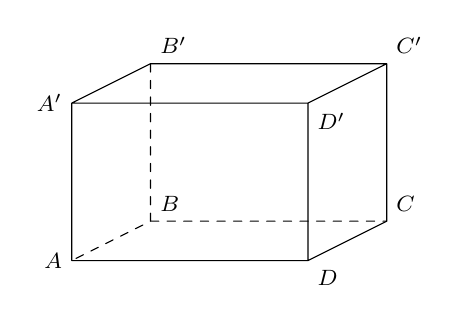
\begin{tikzpicture}[line cap=round, line join=round, font=\footnotesize,>=stealth, scale=1]
				\coordinate (A) at (0,0);
				\coordinate (B) at (1,0.5);
				\coordinate (C) at (4,0.5);
				\coordinate (D) at (3,0);
				\coordinate (A') at (0,2);
				\coordinate (B') at (1,2.5);
				\coordinate (C') at (4,2.5);
				\coordinate (D') at (3,2);
				\draw [dashed] (B')--(B)--(A) (B)--(C);
				\draw
				(A)--(D)--(D')--(A')--cycle
				(A')--(B')--(C')--(D')
				(D)--(C)--(C');
				\foreach \x in {B,C,B',C'} {
					\node[above right] at (\x) {$\x$};
				}
				\foreach \x in {D, D'} {
					\node[below right] at (\x) {$\x$};
				}
				\foreach \x in {A, A'} {
					\node[left] at (\x) {$\x$};	
				}
			\end{tikzpicture}	
		} 
	}
\end{ex}
\begin{ex}%[2H2H1-3]%[Dự án đề cương 3 khối NH24-25-Dot1-Nguyen Huynh]
	(\textit{Trích Đề GHK I Toán 12 năm 2024 – 2025 trường THPT Hùng Vương – TP HCM}) \\
	Cho hình lập phương $ABCD.A'B'C'D'$ (tham khảo hình vẽ dưới đây) có cạnh bằng $a$. 
	\begin{center}
		\begin{tikzpicture}[line cap=round,line join=round,font=\footnotesize,scale=.7]
			\path
			(0,0) coordinate (A)
			(4,0) coordinate (B)
			(-2,-2) coordinate (D)
			($(B)+(D)-(A)$) coordinate (C)
			($(A)!4cm!90:(B)$) coordinate (A') % Co the thay 4cm bang ti so vi tu
			($(A')+(B)-(A)$) coordinate (B')
			($(A')+(D)-(A)$) coordinate (D')
			($(B')+(D')-(A')$) coordinate (C')
			;
			\draw (A')--(B')--(C')--(D')--cycle (D)--(C)--(B) (D)--(D') (C)--(C') (B)--(B');
			\draw[dashed] (A')--(A)--(B) (A)--(D);
			\foreach \i/\g in {A'/90,B'/45,C'/0,D'/180,A/180,B/-45,C/-45,D/-135}
			\draw[fill=black] (\i) circle (1pt) +(\g:.4) node{$\i$};
		\end{tikzpicture}
	\end{center}
	Khi đó $\overrightarrow{AB}\cdot \overrightarrow{A'C'}$ bằng
	\choice
	{$2a^2$}
	{$\dfrac{\sqrt{2}}{2}a^2$}
	{$0$}
	{\True $a^2$}
	\loigiai{
		\begin{center}
			\begin{tikzpicture}[line cap=round,line join=round,font=\footnotesize,scale=.7]
				\path
				(0,0) coordinate (A)
				(4,0) coordinate (B)
				(-2,-2) coordinate (D)
				($(B)+(D)-(A)$) coordinate (C)
				($(A)!4cm!90:(B)$) coordinate (A') % Co the thay 4cm bang ti so vi tu
				($(A')+(B)-(A)$) coordinate (B')
				($(A')+(D)-(A)$) coordinate (D')
				($(B')+(D')-(A')$) coordinate (C')
				;
				\draw (A')--(B')--(C')--(D')--cycle (D)--(C)--(B) (D)--(D') (C)--(C') (B)--(B');
				\draw[dashed] (A')--(A)--(B) (A)--(D);
				\foreach \i/\g in {A'/90,B'/45,C'/0,D'/180,A/180,B/-45,C/-45,D/-135}
				\draw[fill=black] (\i) circle (1pt) +(\g:.4) node{$\i$};
			\end{tikzpicture}
		\end{center}
		Ta có $\overrightarrow{AB}\cdot \overrightarrow{A'C'}=\overrightarrow{AB}\cdot \overrightarrow{AC}=|\overrightarrow{AB}|\cdot |\overrightarrow{AC}|\cdot \cos \left(\overrightarrow{AB}, \overrightarrow{AC}\right)=a\cdot a\sqrt{2} \cdot \cos 45^{\circ}=a^2$.
	}
\end{ex}

\begin{ex}%[2H2N1-2]
	Cho bốn điểm $A, B, C, D$ bất kì trong không gian. Hệ thức đúng là
	\choice
	{$\overrightarrow{AB}+\overrightarrow{CD}=\overrightarrow{AC}+\overrightarrow{DB}$}
	{\True $\overrightarrow{AB}+\overrightarrow{CD}=\overrightarrow{AD}+\overrightarrow{CB}$}
	{$\overrightarrow{AB}+\overrightarrow{CD}=\overrightarrow{AC}+\overrightarrow{BD}$}
	{$\overrightarrow{AB}+\overrightarrow{CD}=\overrightarrow{AD}+\overrightarrow{BC}$}
	\loigiai{
		Ta có
		\allowdisplaybreaks
		\begin{eqnarray*}
			\overrightarrow{AB}+\overrightarrow{CD}&=&\left(\overrightarrow{AD}+\overrightarrow{DB}\right)+\left(\overrightarrow{CB}+\overrightarrow{BD}\right)
			\\
			&=&\overrightarrow{AD}+\overrightarrow{CB}+\left(\overrightarrow{DB}+\overrightarrow{BD}\right)
			\\
			&=&\overrightarrow{AD}+\overrightarrow{CB}+\overrightarrow{0}
			\\
			&=&\overrightarrow{AD}+\overrightarrow{CB}.
		\end{eqnarray*}
	}
\end{ex}

\Closesolutionfile{ans}

\ind{PHẦN II.} \inden{Câu trắc nghiệm đúng sai. Trong mỗi ý a), b), c), d) ở mỗi câu, học sinh chọn đúng hoặc sai.}\\
\setcounter{ex}{0}
\Opensolutionfile{ans}[ans/2H2-Bai1-DS]%--Đặt tên 2D1-Bai1-DS
\begin{ex}%[2H2H1-3]%[Dự án đề cương 3 khối NH24-25-Dot1-Nguyen Huynh]
	\immini{Cho hình chóp $S.ABCD$ có $SA=SB=SC=AB=AC=a$ và $BC=a \sqrt {2}$.
		\choiceTF
		{\True Tam giác $ABC$ vuông tại $A$ và tam giác $SAB$ đều}
		{\True $\overrightarrow{AB} \cdot \overrightarrow{AC}=0$ và $(\overrightarrow{SA}, \overrightarrow{SB})=120^\circ$}
		{ $\overrightarrow{SC} \cdot \overrightarrow{AB}=\dfrac{a^2}{2}$}
		{ $\cos (\overrightarrow{SA}, \overrightarrow{AB})=\dfrac{1}{2}$}
	}
	{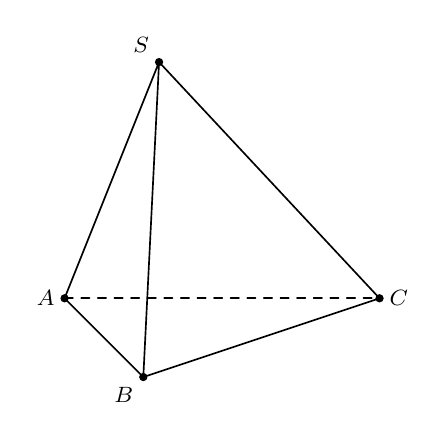
\begin{tikzpicture}[line join=round,line cap=round,line width=.6pt,font=\footnotesize,scale=1]
			\coordinate[label=left:$A$] (A) at (0,0);
			\coordinate[label=below left:$B$] (B) at (1,-1);
			\coordinate[label=right:$C$] (C) at (4,0);
			\coordinate[label=above left:$S$] (S) at (1.2,3);
			\draw (A)--(B)--(C)--(S)--cycle (S)--(B);
			\draw[dashed] (A)--(C);
			\fill (A)circle(1.5pt) (B)circle(1.5pt) (C)circle(1.5pt) (S)circle(1.5pt);
		\end{tikzpicture}
	}
	\loigiai{
		\begin{itemchoice}
			\itemch Đúng. Từ giả thiết, dễ thấy tam giác $ABC$ vuông tại $A$ và tam giác $SAB$ dều.
			\itemch Đúng. Vì tam giác $ABC$ vuông tại $A$ nên $\overrightarrow{AB} \cdot \overrightarrow{AC}=0$ và $(\overrightarrow{SA}, \overrightarrow{SB})=180^\circ-\widehat{SAB}=120^\circ$.
			\itemch Sai.Ta có $\overrightarrow{SC} \cdot \overrightarrow{AB}=(\overrightarrow{S A}+\overrightarrow{AC}) \cdot \overrightarrow{AB}=\overrightarrow{SA} \cdot \overrightarrow{AB}+\overrightarrow{AC} \cdot \overrightarrow{AB}$
			$$=\overrightarrow{SA} \cdot \overrightarrow{AB}=|\overrightarrow{SA}| \cdot|\overrightarrow{AB}| \cdot \cos (\overrightarrow{SA}, \overrightarrow{AB})=|\overrightarrow{SA}| \cdot|\overrightarrow{AB}| \cdot \cos 120^\circ=-\dfrac{a^2}{2}.$$
			\itemch Sai. Do $\cos (\overrightarrow{SA}, \overrightarrow{AB})=\dfrac{\overrightarrow{SC} \cdot \overrightarrow{AB}}{SC \cdot AB}=\dfrac{-\dfrac{a^2}{2}}{a^2}=-\dfrac{1}{2}$.
		\end{itemchoice}
	}
\end{ex}
\begin{ex}%[2H2H1-3]%[Dự án đề cương 3 khối NH24-25-Dot1-Nguyen Huynh]
	\immini{Cho hình chóp tứ giác đều $S.ABCD$ có độ dài tất cả các cạnh đều bằng $a$.
		\choiceTF
		{\True Tứ giác $ABCD$ là hình vuông} 
		{\True Tam giác $SAC$ vuông cân tại $S$}
		{ $(\overrightarrow{SA},\overrightarrow{AC})=45^\circ$}
		{\True $\overrightarrow{SA} \cdot \overrightarrow{AC}=-a^2$}	
	}
	{\begin{tikzpicture}[line join=round,line cap=round,line width=.6pt,font=\footnotesize,scale=0.8]
			\coordinate[label=below left:$B$] (B) at (0,0);
			\coordinate[label=above right:$A$] (A) at (1,.8);
			\coordinate[label=below right:$C$] (C) at (4,0);
			\coordinate[label=above right:$D$] (D) at ($(C)-(B)+(A)$);
			\coordinate[label=below:$O$] (O) at ($(A)!.5!(C)$);
			\coordinate[label=above left:$S$] (S) at ($(O)+(90:4)$);
			\draw (B)--(C)--(D)--(S)--cycle (S)--(C);
			\draw[dashed] (C)--(A)--(D)--(B) (O)--(S)--(A)--(B);
			\fill (A)circle(1.5pt) (B)circle(1.5pt) (C)circle(1.5pt) (D)circle(1.5pt) (S)circle(1.5pt) (O)circle(1.5pt);
		\end{tikzpicture}	
	}
	\loigiai{
		\begin{itemchoice}
			\itemch Đúng. Do $S.ABCD$ làhình chóp tứ giác đều nên $ABCD$ là hình vuông.
			\itemch Đúng. Do tứ giác $ABCD$ là hình vuông có độ dài mỗi cạnh là $a$ nên độ dài đường chéo $AC$ là $a \sqrt{2}$.\\
			Tam giác $SAC$ có $SA=SC=a$ và $AC=\sqrt{2} a$ nên $\triangle SAC$ vuông cân tại $S$.
			\itemch Sai. Vì $\triangle SAC$ vuông cân tại $S$ nên $\widehat{SAC}=45^{\circ}$. Do đó $(\overrightarrow{SA}, \overrightarrow{AC})=180^{\circ}-\widehat{SAC}= 135^{\circ}$. 
			\itemch Đúng. Suy ra $\overrightarrow{SA} \cdot \overrightarrow{AC}=|\overrightarrow{SA}| \cdot |\overrightarrow{AC}| \cdot \cos 135^{\circ}=a \cdot \sqrt{2} a \cdot \left(-\dfrac{\sqrt{2}}{2}\right)=-a^2$.
		\end{itemchoice}
	}
\end{ex}
\begin{ex}%[2H2H1-3]%[Dự án đề cương 3 khối NH24-25-Dot1-Nguyen Huynh]
	\immini{
		Cho hình lập phương $ABCD.A'B'C'D'$ có độ dài cạnh là $a$. Gọi $O$ là giao điểm của $BD$ và $AC$.
		\choiceTF
		{\True $\overrightarrow{A'C}-\overrightarrow{A'A}=\overrightarrow{AB}+\overrightarrow{AD}$}
		{$\overrightarrow{BC'}=\overrightarrow{A'A}+\overrightarrow{B'C'}$}
		{\True $\overrightarrow{C'O}=\overrightarrow{C'A'}-\overrightarrow{OA'}$}
		{$\overrightarrow{A'D} \cdot \overrightarrow{A'B}=0$}
	}{
		\begin{tikzpicture}[scale=0.9,font=\footnotesize,line join=round,line cap=round,>=stealth]
			\def\a{3.5}
			\path (0:0) coordinate (A)
			++(0:\a) coordinate (D)
			++(-130:\a/2) coordinate (C)
			($(A)+(C)-(D)$) coordinate (B)
			($(A)+(90:\a)$) coordinate (A')
			($(B)+(90:\a)$) coordinate (B')
			($(C)+(90:\a)$) coordinate (C')
			($(D)+(90:\a)$) coordinate (D')
			($(A)!0.5!(C)$) coordinate (O)
			;
			\draw[dashed] (B)--(A)--(D) (A)--(A') (A)--(C) (B)--(D);
			\draw (C)--(C') (D)--(D') (B)--(B') (B)--(C)--(D) (A')--(B')--(C')--(D')--cycle;
			\foreach \x/\g in {A/180,B/180,C/0,D/0,A'/180,B'/180,C'/0,D'/0,O/-90}
			\fill (\x) circle (1pt)
			($(\g:4mm)+(\x)$) node {$\x$}; 
		\end{tikzpicture}
	}
	\loigiai{
		\begin{itemchoice}
			\itemch \textbf{Đúng}.\\ 
			Vì $\heva{&\overrightarrow{A'C}-\overrightarrow{A'A}=\overrightarrow{AC} \\
				&\overrightarrow{AB}+\overrightarrow{AD}=\overrightarrow{AC}} \Rightarrow \overrightarrow{A'C}-\overrightarrow{AA'}=\overrightarrow{AB}+\overrightarrow{AD}$.
			\itemch \textbf{Sai}.\\ 
			Vì $\overrightarrow{BC'}=\overrightarrow{BB'}+\overrightarrow{B'C'}=\overrightarrow{AA'}+\overrightarrow{B'C'}$.
			\itemch \textbf{Đúng}.\\ 
			Vì $\overrightarrow{C'O}=\overrightarrow{C'A'}+\overrightarrow{A'O}=\overrightarrow{C'A'}-\overrightarrow{OA'}$.
			\itemch \textbf{Sai}.\\ 
			Xét tam giác $A'BD$ có $A'B=BD=A'D$ (đường chéo hình lập phương) nên tam giác $A'BD$ đều. \\
			Suy ra $\widehat{BA'D}=60^\circ$, do đó $\left(\overrightarrow{A'D}, \overrightarrow{A'B}\right)=60^\circ$.\\
			Ta có $\overrightarrow{A'D} \cdot \overrightarrow{A'B}=\left|\overrightarrow{A'D}\right|\cdot\left|\overrightarrow{A'B}\right|\cdot \cos \left(\overrightarrow{A'D}, \overrightarrow{A'B}\right)=a \sqrt{2} \cdot a \sqrt{2} \cdot \cos 60^{\circ}=a^2$.
		\end{itemchoice}
	}
\end{ex}
\begin{ex}%[2H2V1-3]%[Dự án đề cương 3 khối NH24-25-Dot1-Nguyen Huynh]
	\immini{
		Cho hình lập phương $ABCD.A'B'C'D'$ có cạnh bằng $a$. Đặt $\overrightarrow{AB}=\overrightarrow{x}$, $\overrightarrow{AD}=\overrightarrow{y}$, $\overrightarrow{AA'}=\overrightarrow{z}$. 
		\choiceTF
		{\True $\overrightarrow{AC'}=\overrightarrow{x}+\overrightarrow{y}+\overrightarrow{z}$}
		{$\overrightarrow{A'B}=\overrightarrow{x}+\overrightarrow{z}$}
		{Góc giữa vectơ $\overrightarrow{BA'}$ và vectơ $\overrightarrow{A'C'}$ bằng $60^{\circ}$}
		{\True Gọi $M$ là trung điểm của $BC$. Độ dài vectơ $\overrightarrow{A'M}$ bằng $\dfrac{3a}{2}$}}
	{\begin{tikzpicture}[scale=0.8,font=\footnotesize,line join=round,line cap=round,>=stealth]
			\def\a{3.5}
			\path (0:0) coordinate (A)
			++(0:\a) coordinate (D)
			++(-130:\a/2) coordinate (C)
			($(A)+(C)-(D)$) coordinate (B)
			($(A)+(90:\a)$) coordinate (A')
			($(B)+(90:\a)$) coordinate (B')
			($(C)+(90:\a)$) coordinate (C')
			($(D)+(90:\a)$) coordinate (D')
			($(A)!0.5!(C)$) coordinate (O)
			;
			\draw[dashed] (B)--(A)--(D) (A)--(A');
			\draw (C)--(C') (D)--(D') (B)--(B') (B)--(C)--(D) (A')--(B')--(C')--(D')--cycle;
			\foreach \x/\g in {A/180,B/180,C/0,D/0,A'/180,B'/180,C'/0,D'/0}
			\fill (\x) circle (1pt)
			($(\g:4mm)+(\x)$) node {$\x$}; 
	\end{tikzpicture}}
	\loigiai{
		\begin{center}
			\begin{tikzpicture}[scale=0.8,font=\footnotesize,line join=round,line cap=round,>=stealth]
				\def\a{3.5}
				\path (0:0) coordinate (A)
				++(0:\a) coordinate (D)
				++(-130:\a/2) coordinate (C)
				($(A)+(C)-(D)$) coordinate (B)
				($(A)+(90:\a)$) coordinate (A')
				($(B)+(90:\a)$) coordinate (B')
				($(C)+(90:\a)$) coordinate (C')
				($(D)+(90:\a)$) coordinate (D')
				($(A)!0.5!(C)$) coordinate (O)
				($(B)!0.5!(C)$) coordinate (M)
				;
				\draw[dashed] (B)--(A)--(D) (C')--(A)--(A')--(B) (A)--(M)--(A');
				\draw (C)--(C') (D)--(D') (B)--(B') (B)--(C)--(D) (A')--(C') (A')--(B')--(C')--(D')--cycle;
				\foreach \x/\g in {A/180,B/180,C/0,D/0,A'/180,B'/180,C'/0,D'/0,M/-90}
				\fill (\x) circle (1pt)
				($(\g:4mm)+(\x)$) node {$\x$}; 
			\end{tikzpicture}
		\end{center}
		\begin{itemchoice}
			\itemch \textbf{Đúng}.\\
			Theo quy tắc hình hộp ta có $\overrightarrow{AC'}=\overrightarrow{AB}+\overrightarrow{AD}+\overrightarrow{AA'}=\overrightarrow{x}+\overrightarrow{y}+\overrightarrow{z}$.
			\itemch \textbf{Sai}.\\
			Theo quy tắc $3$ điểm ta có $\overrightarrow{A'B}=\overrightarrow{AB}-\overrightarrow{AA'}=\overrightarrow{x}-\overrightarrow{z}$.
			\itemch \textbf{Sai}.\\
			Vì hình lập phương có cạnh bằng $a$ nên $A'B=A'C'=C'B=a \sqrt{2}$, do đó tam giác $A'BC'$ đều, nên $\widehat{BA'C'}=60^{\circ} \Rightarrow\left(\overrightarrow{BA'}, \overrightarrow{A'C'}\right)=180^{\circ}-\left(\overrightarrow{A'B}, \overrightarrow{A'C'}\right)=180^{\circ}-60^{\circ}=120^{\circ}$.
			\itemch \textbf{Đúng}.\\
			Ta có $ABCD.A'B'C'D'$ là hình lập phương nên $AA'\perp(ABCD) \Rightarrow AA'\perp AM$, suy ra tam giác $AA'M$ vuông tại $A$.\\
			Có $\left|\overrightarrow{A'M}\right|=A'M=\sqrt{AA'^2+AM^2}=\sqrt{AA'^2+AB^2+BM^2}=\sqrt{a^2+a^2+\dfrac{a^2}{4}}=\dfrac{3a}{2}$.
		\end{itemchoice}
	}
\end{ex}


\begin{ex}%[2H2V1-2]%[Dự án đề cương 3 khối NH24-25-Dot1-Nguyen Huynh]
	\immini{
		Cho tứ diện đều $ABCD$. Gọi $G$ là trọng tâm của tam giác $BCD$, gọi $I$ là điểm thuộc đoạn $AG$ và thỏa mãn $AI=3IG$. 
		\choiceTF
		{\True $\overrightarrow{GB}+\overrightarrow{GC}+\overrightarrow{GD}=\overrightarrow{0}$}
		{$\overrightarrow{AG}=\dfrac{1}{3} \overrightarrow{AB}+\dfrac{2}{3} \overrightarrow{AC}+\dfrac{2}{3} \overrightarrow{AD}$}
		{\True $\overrightarrow{CG}=\dfrac{1}{3} \overrightarrow{AB}-\dfrac{2}{3} \overrightarrow{AC}+\dfrac{1}{3} \overrightarrow{AD}$}
		{\True $\overrightarrow{IA}+\overrightarrow{IB}+\overrightarrow{IC}+\overrightarrow{ID}=\overrightarrow{0}$}
	}{
		\begin{tikzpicture}[scale=0.8,font=\footnotesize,line join=round,line cap=round,>=stealth]
			\def\a{4}
			\def\h{4}
			\path (0:0) coordinate (B)
			++(0:\a) coordinate (D)
			++(-150:4*\a/5) coordinate (C)
			($(D)!0.5!(B)$) coordinate (M)
			($(C)!2/3!(M)$) coordinate (G)
			($(G)+(90:\h)$) coordinate (A)
			($(A)!2/3!(G)$) coordinate (I)
			;
			\draw (C)--(A) (B)--(A)
			(A)--(D) (B)--(C)--(D);
			\draw[dashed] (D)--(B) (A)--(G) (C)--(M);
			\foreach \x / \goc in {A/90,B/180,C/-135,G/0,I/0,D/0}
			\fill (\x) circle (1.0pt)
			($(\x)+(\goc:3mm)$) node {$\x$};
		\end{tikzpicture}
	}
	\loigiai{
		\begin{itemchoice}
			\itemch \textbf{Đúng}.\\ 
			Theo tính chất trọng tâm, ta có $\overrightarrow{GB}+\overrightarrow{GC}+\overrightarrow{GD}=\overrightarrow{0}$.
			\itemch \textbf{Sai}.\\
			Theo quy tắc trọng tâm, ta có
			\[
			\overrightarrow{AB}+\overrightarrow{AC}+\overrightarrow{AD}=3\overrightarrow{AG} \Leftrightarrow \overrightarrow{AG}=\dfrac{1}{3} \overrightarrow{AB}+\dfrac{1}{3} \overrightarrow{AC}+\dfrac{1}{3} \overrightarrow{AD}.
			\]
			\itemch \textbf{Đúng}.\\
			\[
			\overrightarrow{CG}=\overrightarrow{AG}-\overrightarrow{AC}=\dfrac{1}{3} \overrightarrow{AB}+\dfrac{1}{3} \overrightarrow{AC}+\dfrac{1}{3} \overrightarrow{AD}-\overrightarrow{AC}=\dfrac{1}{3} \overrightarrow{AB}-\dfrac{2}{3} \overrightarrow{AC}+\dfrac{1}{3} \overrightarrow{AD}.
			\]
			\itemch \textbf{Đúng}.\\
			Vì $I$ là điểm thuộc đoạn $AG$ và $AI=3IG\Rightarrow \overrightarrow{AI}=3\overrightarrow{IG}$, mà $G$ là trọng tâm tam giác $BCD$ nên 
			\allowdisplaybreaks
			\begin{eqnarray*}
				&&\overrightarrow{IB}+\overrightarrow{IC}+\overrightarrow{ID}=3\overrightarrow{IG} \\
				&\Leftrightarrow& \overrightarrow{IB}+\overrightarrow{IC}+\overrightarrow{ID}=\overrightarrow{AI} \\
				&\Leftrightarrow& \overrightarrow{IB}+\overrightarrow{IC}+\overrightarrow{ID}=-\overrightarrow{IA}\\
				&\Leftrightarrow& \overrightarrow{IA}+\overrightarrow{IB}+\overrightarrow{IC}+\overrightarrow{ID}=\overrightarrow{0}.
			\end{eqnarray*}
		\end{itemchoice}
	}
\end{ex}
\Closesolutionfile{ans}


\ind{PHẦN III.} \inden{Câu trắc nghiệm trả lời ngắn. }\\
\setcounter{ex}{0}
\Opensolutionfile{ans}[ans/2H2-Bai1-DS]%--Đặt tên 2D1-Bai1-DS
%%%==============Bai_BT2==============%%%
\begin{ex}%[2H2V1-2]%[Dự án đề cương 3 khối NH24-25-Dot1-Nguyen Huynh]
	\immini{
		Cho hình lăng trụ $ABC.A'B'C'$ có $M$ là trung điểm $BB'$ (tham khảo hình vẽ). Biết $\overrightarrow{AM}=m\overrightarrow{CB}+n\overrightarrow{CA}+p\overrightarrow{CC'}$ ($m$, $n$, $p\in \mathbb{R}$). Tính $m+n+p$.
		
	}{
		\begin{tikzpicture}[line join = round, line cap = round,font=\footnotesize,>=stealth,scale=.7]
			\path
			(0:0) coordinate (A)
			(0:6) coordinate (C)
			(-26:2.5) coordinate (B)
			(76:4) coordinate (A')
			($(A')+(B)$) coordinate (B')
			($(A')+(C)$) coordinate (C')
			($(B)!.5!(B')$) coordinate (M);
			\draw (A')--(B')--(C')--cycle (A')--(A) (B')--(B) (C')--(C) (A)--(B)--(C);
			\draw[dashed] (A)--(C);
			\foreach \x/\g in {A/180,B/-90,C/-30,A'/180,B'/-160,C'/-30,M/0}\draw[fill=white] (\x) circle (1.0pt)+(\g:.3)node{$\x$};
		\end{tikzpicture}
	}
	\shortans[oly]{$0{,}5$}
	\loigiai{
		Ta có 
		\begin{eqnarray*}
			\overrightarrow{AM}&=&\overrightarrow{CM}-\overrightarrow{CA}=\dfrac{1}{2}\overrightarrow{CB}+\dfrac{1}{2}\overrightarrow{CB}+\dfrac{1}{2}\overrightarrow{CC'}-\overrightarrow{CA}\\
			&=&\overrightarrow{CB}-\overrightarrow{CA}+\dfrac{1}{2}\overrightarrow{CC'}.
		\end{eqnarray*}
		Vậy $m=1$, $n=-1$ và $p=\dfrac{1}{2}$.\\
		Suy ra $m+n+p=0{,}5$.
	}
\end{ex}
\begin{ex}%[2H2V1-4]%[Dự án đề cương 3 khối NH24-25-Dot1-Nguyen Huynh]
	(\textit{Trích Đề ôn tập GHK I Toán 12 năm 2024 – 2025 trường THPT Bùi Thị Xuân – TP HCM}) \\
	\immini{Ba lực $\overrightarrow{F}_1$, $\overrightarrow{F}_2$, $\overrightarrow{F}_3$ cùng tác động vào một vật có phương đôi một vuông góc và có độ lớn lần lượt là $2N$, $3N$, $5N$. Độ lớn hợp lực $\overrightarrow{F}=\overrightarrow{F}_1+\overrightarrow{F}_2+\overrightarrow{F}_3$ bằng bao nhiêu Niuton? (làm tròn kết quả đến hàng phần trăm).}
	{\begin{tikzpicture}[scale=0.7, font=\footnotesize, line join=round, line cap=round]
			%---------------------------
			\foreach \x\y\t in {0/0/O, -2/-1.3/B, 4/0/A,0/3/C}
			\coordinate (\t) at (\x,\y);
			\coordinate (D) at ($(A)+(B)$);
			\coordinate (E) at ($(C)+(D)$);
			%\coordinate (x) at (intersection of A--O and E--D);
			\path (O)--(A)node[pos=0.5,above]{$\overrightarrow{F_1}$};
			\path (O)--(B)node[pos=0.5,above left]{$\overrightarrow{F_2}$};
			\path (O)--(C)node[pos=0.5,left]{$\overrightarrow{F_3}$};			
			\draw[->] (O)--(A);
			\draw[->] (O)--(B);
			\draw[->] (O)--(C);
			\draw pic[draw,angle radius=2mm] {right angle = A--O--B};
			\draw pic[draw,angle radius=2mm] {right angle = A--O--C};
			\draw pic[draw,angle radius=2mm] {right angle = C--O--B};
			\foreach \t\g in {O/-90}
			\draw[fill=black] (\t)circle(0.6pt) +(\g:12pt)node{$\t$};
	\end{tikzpicture}}
	\shortans[oly]{6,16}
	\loigiai{
		Ta có $\left |\overrightarrow{F}\right |=\left |\overrightarrow{F}_1+\overrightarrow{F}_2+\overrightarrow{F}_3\right |=\sqrt{\left |\overrightarrow{F}_1\right |^2+\left |\overrightarrow{F}_2\right |^2+\left |\overrightarrow{F}_3\right |^2}=\sqrt{2^2+3^2+5^2}=\sqrt{38}\approx 6{,}16$.
	}
\end{ex}
%%%==============HetBai_BT2==============%%%
\begin{ex}%[2H2V1-2][Dự án đề cương 3 khối NH24-25-Dot1-Nguyen Huynh]
	(\textit{Trích Đề GHK I Toán 12 năm 2024 – 2025 trường THPT Lê Trọng Tấn – TP HCM}) \\
	Cho tứ diện $A B C D$. Gọi $M$, $N$, $P$, $G$ lần lượt là trọng tâm các tam giác $A B C$, $A C D$, $A B D$ và $B C D$, biết $\overrightarrow{A G}=x \overrightarrow{A M}+y \overrightarrow{A N}+z \overrightarrow{A P}$. Tính $x+y+z$.
	\shortans[oly]{1,5}
	\loigiai{
		Vì $G$ là trọng tâm tam giác $BCD$ nên $\overrightarrow{AG}=\dfrac{1}{3} \left( \overrightarrow{AB}+\overrightarrow{AC}+\overrightarrow{AD} \right)$.\qquad (1)\\
		Vì $M$ là trọng tâm tam giác $ABC$ nên $\overrightarrow{AM}=\dfrac{1}{3} \left( \overrightarrow{AA}+\overrightarrow{AB}+\overrightarrow{AC} \right)= \dfrac{1}{3} \left( \overrightarrow{AB}+\overrightarrow{AC} \right)$.\\
		Vì $N$ là trọng tâm tam giác $ACD$ nên $\overrightarrow{AN}=\dfrac{1}{3} \left( \overrightarrow{AA}+\overrightarrow{AC}+\overrightarrow{AD} \right)= \dfrac{1}{3} \left( \overrightarrow{AC} + \overrightarrow{AD}\right)$.\\
		Vì $P$ là trọng tâm tam giác $ABD$ nên $\overrightarrow{AP}=\dfrac{1}{3} \left( \overrightarrow{AA}+\overrightarrow{AB}+\overrightarrow{AD} \right)= \dfrac{1}{3} \left( \overrightarrow{AB}+\overrightarrow{AD} \right)$.\\
		Suy ra \allowdisplaybreaks
		$ \begin{aligned}[t]
			&\overrightarrow{AM}+\overrightarrow{AN}+\overrightarrow{AP}=\dfrac{1}{3} \left( 2\overrightarrow{AB} + 2\overrightarrow{AC} +2\overrightarrow{AD} \right) \\
			&\Leftrightarrow \dfrac{1}{2} \left( \overrightarrow{AM}+\overrightarrow{AN}+\overrightarrow{AP} \right)=\dfrac{1}{3} \left( \overrightarrow{AB} + \overrightarrow{AC} +\overrightarrow{AD} \right).\qquad (2)
		\end{aligned} $ \\
		Từ (1) và (2) ta được $\overrightarrow{AG}=\dfrac{1}{2} \left( \overrightarrow{AM}+\overrightarrow{AN}+\overrightarrow{AP} \right)$ nên $x=y=z=\dfrac{1}{2}$.\\
		Vậy $x+y+z=\dfrac{3}{2}$.
	}
\end{ex}



\begin{ex}%[2H2V1-3]%[Dự án đề cương 3 khối NH24-25-Dot1-Nguyen Huynh]
	Cho tứ diện đều $S. ABC$ cạnh $a$, $M$ là trung điểm của cạnh $BC$. Tính $\cos \left(\overrightarrow{AM}, \overrightarrow{SB}\right)$ (Kết quả làm tròn đến hàng phần trăm).
	
	\shortans[oly]{0,29}
	\loigiai{
		\begin{center}
			\begin{tikzpicture}[scale=1,font=\footnotesize,line join=round,line cap=round,>=stealth]
				\def\a{4}
				\def\h{4}
				\path (0:0) coordinate (A)
				++(0:\a) coordinate (B)
				++(-150:4*\a/5) coordinate (C)
				($(A)!0.5!(B)$) coordinate (N)
				($(C)!2/3!(N)$) coordinate (H)
				($(H)+(90:\h)$) coordinate (S)
				($(C)!0.5!(B)$) coordinate (M)
				;
				\draw (C)--(A) (C)--(B)
				(A)--(S) (B)--(S) (C)--(S);
				\draw[dashed] (A)--(B) (S)--(H) (A)--(M);
				\foreach \x / \goc in {A/180,B/0,C/-135,H/40,M/-45,S/90}
				\fill (\x) circle (1.0pt)
				($(\x)+(\goc:3mm)$) node {$\x$};
			\end{tikzpicture}
		\end{center} 
		Ta có
		\allowdisplaybreaks
		\begin{align*}
			\overrightarrow{AM} \cdot \overrightarrow{SB}&=(\overrightarrow{SM}-\overrightarrow{SA}) \cdot \overrightarrow{SB}\\
			&=\overrightarrow{SM} \cdot \overrightarrow{SB}-\overrightarrow{SA} \cdot \overrightarrow{SB}\\
			&=SM\cdot SB\cdot \cos \widehat{BSM}-SA\cdot SB\cdot \cos \widehat{ASB}\\
			&=\dfrac{a \sqrt{3}}{2} \cdot a \cdot \cos 30^{\circ}-a \cdot a \cdot \cos 60^{\circ} \\
			&=\dfrac{a^2}{4}.
		\end{align*}
		Suy ra \[
		\cos \left(\overrightarrow{AM}, \overrightarrow{SB}\right)=\dfrac{\overrightarrow{AM} \cdot \overrightarrow{SB}}{AM\cdot SB}=\dfrac{\dfrac{a^2}{4}}{\dfrac{a \sqrt{3}}{2} \cdot a}=\dfrac{\sqrt{3}}{6} \approx 0{,}29.\]
	}
\end{ex}

\begin{ex}%[2H2H1-3]
	Cho hình lập phương $ABCD.A’B’C’D’$ có cạnh bằng $a$. Gọi $M$, $N$ lần lượt là trung điểm của $A’D’$ và $C’D’$. Tích vô hướng $\overrightarrow{MN}\cdot \overrightarrow{C'B}=na^2$ ($n$ là số thập phân). Giá trị của $n$ bằng bao nhiêu?
	\shortans[oly]{$-0{,}5$}
	\loigiai{
		Vì $MN \parallel A'C'$ nên $(\vec{MN}, \vec{C'B}) = (\vec{A'C'}, \vec{C'B}) = 180^\circ - \widehat{A'C'B} = 120^\circ$.
		
		Ta có $MN=\dfrac{a\sqrt{2}}{2}$, $C'B= a\sqrt{2}$. Suy ra 
		$$\vec{MN}\cdot \vec{C'B}= \left|\vec{MN}\right|\cdot \left|\vec{C'B}\right|
		\cdot \cos(\vec{MN}, \vec{C'B})=\dfrac{a\sqrt{2}}{2}\cdot a\sqrt{2}\cdot\cos 120^\circ=-0{,}5a^2.$$
		
		Vậy $n = - 0{,}5$.
		
		\begin{center}
			\begin{tikzpicture}[line join=round, line cap = round, >=stealth, scale=.8,font=\footnotesize,transform shape]
				\foreach \x/\y/\z/\g in
				{
					0/0/A/-135, 1.8/1/D/180, 4.8/1/C/0, 3/0/B/-45,
					0/3/A'/180, 1.8/4/D'/90, 4.8/4/C'/45, 3/3/B'/90
				}
				\draw[fill=black] (\x,\y) circle(1pt) coordinate (\z) ($(\z)+(\g:3.5mm)$) node{$\z$};
				\draw (B')--(C')--(B)--(B')--(A')--(D')--(C')--(C) (A')--(A)--(B)--(C) (A')--(C')--(B)--(A');
				\draw[dashed] (A)--(D')--(D)--(A) (C')--(D)--(C);
				
				\path 
				($(A')!.5!(D')$) coordinate (M) node [above]{$M$}
				($(D')!.5!(C')$) coordinate (N) node [above]{$N$}
				;
				\draw[-{Stealth[length=2.5mm]},thick] (M)--(N);
			\end{tikzpicture}
		\end{center}
	}
\end{ex}
\Closesolutionfile{ans}


\ind{PHẦN IV.} \inden{Tự luận.}\\
\setcounter{ex}{0}
%%%==============BT_2==============%%%
\begin{ex}%[2H2H1-2]%[Dự án đề cương 3 khối NH24-25-Dot1-Nguyen Huynh]
	Cho hình chóp đều $S. ABCD$ có cạnh đáy $a$ và đường cao $h$. Gọi  $M$, $N$, $P$, $Q$ lần lượt là trung điểm của các cạnh bên $SA$, $SB$, $SC$, $SD$ và $O$, $H$ lần lượt là tâm của các hình vuông $ABCD$, $MNPQ$.
	\begin{center}
		\begin{tikzpicture}[line join=round, line cap=round,thick, >=stealth, scale=0.8]
			\coordinate (A) at (0,0);
			\coordinate (B) at (2,-2);
			\coordinate (D) at (5,0);
			\coordinate (C) at ($(B)+(D)-(A)$);
			\coordinate (O) at ($(A)!0.5!(C)$);
			\coordinate (S) at ($(O)+(0,7)$);
			\coordinate (M) at ($(A)!0.5!(S)$);
			\coordinate (N) at ($(B)!0.5!(S)$);
			\coordinate (P) at ($(S)!0.5!(C)$);
			\coordinate (Q) at ($(S)!0.5!(D)$);
			\coordinate (H) at ($(M)!0.5!(P)$);
			\draw(S)--(A) (S)--(B) (S)--(C) (A)--(B) (B)--(C) (N)--(P);
			\draw[dashed,thin](A)--(C) (A)--(D) (C)--(D) (S)--(D) (S)--(O) (B)--(D) (M)--(Q)--(P);
			\draw[red, ->, very thick] (M)--(N);
			\draw[red, ->, very thick] (M)--(S);
			\draw[red, ->, dashed, very thick] (M)--(P);
			\pic[draw,thin,angle radius=2mm] {right angle = S--O--D} pic[draw,thin,angle radius=2mm] {right angle = S--O--A};
			\foreach \i/\g in {S/90,A/180,B/-90,C/-90,D/0,O/-90, M/180, N/210, P/0, Q/45, H/45}{\draw[fill=black](\i) circle (1pt) ($(\i)+(\g:3mm)$) node[scale=0.7]{$\i$};}
		\end{tikzpicture}
	\end{center}
	\begin{enumerate}
		\item Trong những vectơ khác $\overrightarrow{0}$, có điểm đầu và điểm cuối là những điểm cho trên hình, hãy liệt kê các vectơ
		\begin{itemize}
			\item Cùng hướng với $\overrightarrow{MN}$.
			\item Bằng $\overrightarrow{MN}$.
		\end{itemize}
		\item Tìm độ dài các vectơ $\overrightarrow{MP}$, $\overrightarrow{MS}$ theo $a$ và $h$.
	\end{enumerate}
	\loigiai{
		\begin{enumerate}
			\item Trong những vectơ khác $\overrightarrow{0}$, có điểm đầu và điểm cuối là những điểm cho trên hình, các vectơ
			\begin{itemize}
				\item Cùng hướng với $\overrightarrow{MN}$ là $\overrightarrow{AB}$, $\overrightarrow{QP}$, $\overrightarrow{DC}$.
				\item Bằng $\overrightarrow{MN}$ là $\overrightarrow{QP}$.
			\end{itemize}
			\item Tìm độ dài các vectơ $\overrightarrow{MP}$, $\overrightarrow{MS}$ theo $a$ và $h$. \\
			Do $ABCD$ là hình vuông nên $AC = a \sqrt{2}$. \\
			Ta có $MP$ là đường trung bình của $\triangle SAC \Rightarrow MP = \dfrac{1}{2} AC = \dfrac{a \sqrt{2}}{2}$. \\
			Xét $\triangle SOA$ vuông tại $O$ ta có
			\begin{eqnarray*}
				SA^2 &=& SO^2 + AO^2 \\
				& = & SO^2 + \left (\dfrac{AC}{2}\right)^2 = h^2 + \left (\dfrac{a \sqrt{2}}{2}\right)^2 = h^2 + \dfrac{a^2}{2} = \dfrac{2h^2 + a^2}{2}.
			\end{eqnarray*}
			Do $M$ là trung điểm $SA$ nên $MS = \dfrac{SA}{2} = \dfrac{1}{2}\sqrt{\dfrac{2h^2 + a^2}{2}}$.
		\end{enumerate}
	}
\end{ex}
\begin{ex}%[2H2H1-2]%[Dự án đề cương 3 khối NH24-25-Dot1-Nguyen Huynh]
	Cho tứ diện $OABC$. Tìm các vectơ
	\begin{multicols}{2}
		\begin{enumerate}
			\item $\overrightarrow{OA}+\overrightarrow{AB}-\overrightarrow{OC}$;
			\item $\overrightarrow{OA}+\overrightarrow{OB}+\overrightarrow{OC}$.
		\end{enumerate}
	\end{multicols}	
	\loigiai{
		\immini{
			\begin{enumerate}
				\item $\overrightarrow{OA}+\overrightarrow{AB}-\overrightarrow{OC}=\overrightarrow{OB}-\overrightarrow{OC}=\overrightarrow{CB}$.
				\item Vẽ hình hộp $OADB.CFEK$.\\
				Ta có $\overrightarrow{OA}+\overrightarrow{OB}+\overrightarrow{OC}=\overrightarrow{OE}$.
			\end{enumerate}			
		}{
			\begin{tikzpicture}[scale=0.5, font=\footnotesize,line join=round, line cap=round, >=stealth]
				\path 
				(0,0) coordinate (B)
				++(-130:3) coordinate (O)
				++(0:4) coordinate (A)
				($(B)+(A)-(O)$) coordinate (D);
				\foreach \i/\t in {B/F,O/C,A/K,D/E}{
					\coordinate (\t) at ($(\i)+(1.5,4)$);}
				\draw (C)--(F)--(E)--(K)--(C)--(O)--(A)--cycle
				(K)--(A)--(D)--(E);
				\draw[dashed,thin] (D)--(B)--(F) (C)--(B)--(O)  (B)--(A);
				\foreach \i/\g in {B/180,O/180,A/0,D/0,F/90,C/90,K/90,E/90}
				\fill[black] (\i) circle(1pt)+(\g:0.4)node[scale=1]{$\i$};
			\end{tikzpicture}
		}		
	}	
\end{ex}
\begin{ex}%[2H2H1-3]%[Dự án đề cương 3 khối NH24-25-Dot1-Nguyen Huynh]
	Cho tứ diện $A B C D$. Chứng minh rằng
	\begin{enumerate}[a)]	
		\item   $\overrightarrow{A B} \cdot \overrightarrow{C D}=\overrightarrow{A C} \cdot \overrightarrow{C D}+\overrightarrow{B C} \cdot \overrightarrow{D C}$;
		\item  $\overrightarrow{A B} \cdot \overrightarrow{C D}+\overrightarrow{A C} \cdot \overrightarrow{D B}+\overrightarrow{A D} \cdot \overrightarrow{B C}=0$.	
	\end{enumerate}
	\loigiai{
		\immini{\begin{enumerate}[a)]	
				\item   $\overrightarrow{A C} \cdot \overrightarrow{C D}+\overrightarrow{B C} \cdot \overrightarrow{D C}= \overrightarrow{C D}\left(\overrightarrow{A C} -\overrightarrow{B C}  \right)=\overrightarrow{A B} \cdot \overrightarrow{C D} $;
				\item  	
				\begin{eqnarray*}
					&&\overrightarrow{A B} \cdot \overrightarrow{C D}+\overrightarrow{A C} \cdot \overrightarrow{D B}+\overrightarrow{A D} \cdot \overrightarrow{B C}\\
					&= & \overrightarrow{A C} \cdot \overrightarrow{C D}+\overrightarrow{B C} \cdot \overrightarrow{D C}+\overrightarrow{A C} \cdot \overrightarrow{D B}+\overrightarrow{A D} \cdot \overrightarrow{B C}\\
					&=& \overrightarrow{A C} \cdot \left(\overrightarrow{C D} +\overrightarrow{D B}\right)+\overrightarrow{B C}\cdot\left(\overrightarrow{A D}+\overrightarrow{DC} \right)=0
				\end{eqnarray*}
		\end{enumerate}}{\begin{tikzpicture}[font=\footnotesize,line join=round, line cap=round, >=stealth,scale=0.7] 
				\def\a{4}
				\path 	(0:0) coordinate (B)
				++(0:\a) coordinate (D)
				++(-120:\a/2) coordinate (C)
				($(B)+(70:\a)$) coordinate (A);
				\draw[dashed,thick] 	(B)--(D);
				\draw[thick] 			(B)--(A)--(D) (A)--(C)
				(B)--(C)--(D);
				\foreach \x/\g in {A/90,B/180,C/-45,D/0}
				\fill[black] 	(\x) circle (1pt)
				($(\g:3mm)+(\x)$) node {$\x$};
				%Hình chóp S.ABC có SA vuông góc đáy	
		\end{tikzpicture}}		
	}
\end{ex}
%===>Bài tập 3
\begin{ex}%[2H2H1-2]%[Dự án đề cương 3 khối NH24-25-Dot1-Nguyen Huynh]
	Ba lực có điểm đặt tại một đỉnh của hình lập phương, cùng phương với ba cạnh và cùng có cường độ là $5$ N. Tính cường độ của hợp lực.
	\loigiai{
		\begin{center}
			\begin{tikzpicture}[scale=0.6, font=\footnotesize, line join=round, line cap=round, >=Stealth]
				\path 
				(0:0) coordinate (B')
				(0:4) coordinate (C')
				($(B')+(45:2)$) coordinate (A')
				($(A')+(C')-(B')$) coordinate (D')
				($(A')+(90:3)$) coordinate (A)
				($(B')+(90:3)$) coordinate (B)
				($(C')+(90:3)$) coordinate (C)
				($(D')+(90:3)$) coordinate (D)
				
				;
				\draw[->,dashed] (A)--(A');
				\draw[->] (A)--(B);
				\draw[->] (A)--(D);
				\draw[dashed] (B')--(A')--(D')
				;
				\draw (B)--(C)--(D)--(D')--(C')--(B')--(B) (C)--(C')
				;
				\foreach \x/\g in {A/170,B/170,C/0,D/0,A'/170,B'/170,C'/0,D'/0}
				\draw[fill=black] 	(\x) circle (.5pt)
				($(\g:.3)+(\x)$) node {$\x$};	
			\end{tikzpicture}
		\end{center}
		Gọi $\overrightarrow{F_1}=\overrightarrow{AB}$; $\overrightarrow{F_2}=\overrightarrow{AB}$; $\overrightarrow{F_3}=\overrightarrow{AA'}$ là ba lực có điểm đặt tại đỉnh $A$ của hình lập phương. Khi đó hợp lực là 
		$\begin{aligned}[t]
			\overrightarrow{F}	&= \overrightarrow{AB} + \overrightarrow{AD} + \overrightarrow{AA'}\\
			&= \overrightarrow{AC'}.
		\end{aligned}$
		\begin{itemize}
			\item Trong $\triangle ADD'$ có $\begin{aligned}[t]
				AD'^2	&= AD^2 + DD'^2 \\
				&= 5^2+5^2 = 50.
			\end{aligned}$
			\item Trong $\triangle AD'C'$ có $\begin{aligned}[t]
				AC'^2	&= AD'^2 + D'C'^2 \\
				&= 50+5^2 = 75.
			\end{aligned}$
		\end{itemize}
		Vậy cường độ của hợp lực $\overrightarrow{F}$ là $\sqrt{75}$ N.
	}
\end{ex}
%===>Bài tập 4
\begin{ex}%[2H2H1-2]%[Dự án đề cương 3 khối NH24-25-Dot1-Nguyen Huynh]
	Cho hình chóp $S.ABCD$. Gọi $I$ là trọng tâm của tam giác $ABC$ và $J$ là trọng tâm tam giác $ADC$. Chứng minh $2\overrightarrow{SA}+\overrightarrow{SB}+2\overrightarrow{SC}+\overrightarrow{SD}=3(\overrightarrow{SI}+\overrightarrow{SJ})$.
	\loigiai{
		\begin{center}
			\begin{tikzpicture}[scale=1, font=\footnotesize, line join=round, line cap=round, >=Stealth]
				\def\a{4}
				\path 
				(0:0) coordinate (B)
				(0:\a) coordinate (C)
				($(C)+(45:\a/2)$) coordinate (D)
				($(B)+(45:\a/3)$) coordinate (A)
				($(B)+(70:\a)$) coordinate (S)
				(intersection of A--C and B--D) coordinate (O)
				($(A)!.5!(B)$) coordinate (K)
				(intersection of K--C and B--D) coordinate (I)
				($(C)!.5!(D)$) coordinate (H)
				(intersection of A--H and B--D) coordinate (J)
				;
				\draw[->,dashed] (S)--(A);
				\draw[->,dashed] (S)--(I);
				\draw[->,dashed] (S)--(J);
				\draw[->] (S)--(C);
				\draw[->] (S)--(B);
				\draw[->] (S)--(D)	;
				\draw[dashed] 	(A)--(B) (A)--(D)--(B) (A)--(C) (S)--(O) (C)--(I) (A)--(J)
				;
				\draw (B)--(C)--(D)
				;
				\foreach \x/\g in {A/180,B/180,C/0,D/0,S/90,O/-90,I/-90,J/-90}
				\draw[fill=black] 	(\x) circle (.5pt)
				($(\g:.2)+(\x)$) node {$\x$};	
			\end{tikzpicture}
		\end{center}
		Ta có $3\overrightarrow{SI} = \overrightarrow{SA} + \overrightarrow{SB} +\overrightarrow{SC}$.\\
		và $3\overrightarrow{SJ}=\overrightarrow{SA} + \overrightarrow{SB} + \overrightarrow{SD}$.\\
		Từ đó suy ra $$2\overrightarrow{SA}+\overrightarrow{SB}+2\overrightarrow{SC}+\overrightarrow{SD}=3(\overrightarrow{SI}+\overrightarrow{SJ}).$$
	}
\end{ex}
%===>Bài tập 5
\begin{ex}%[2H2H1-2]%[Dự án đề cương 3 khối NH24-25-Dot1-Nguyen Huynh]
	Cho hình lăng trụ tam giác $ABC.A'B'C'$ có $\overrightarrow{AA'}=\overrightarrow{a}$, $\overrightarrow{AB}=\overrightarrow{b}$, $\overrightarrow{AC}=\overrightarrow{c}$.
	Chứng minh rằng $\overrightarrow{B'C}=\overrightarrow{c}-\overrightarrow{a}-\overrightarrow{b}$ và $\overrightarrow{BC'}=\overrightarrow{a}-\overrightarrow{b}+\overrightarrow{c}$.
	\loigiai{
		\begin{center}
			\begin{tikzpicture}[scale=1, font=\footnotesize, line join=round, line cap=round]
				\foreach \x\y\t in {0.5/3.4/A',0/0/A,1.5/-1/B,3.5/0/C}
				\coordinate (\t) at (\x,\y);
				\coordinate (B') at ($(B)+(A')-(A)$);
				\coordinate (C') at ($(C)+(A')-(A)$);
				\foreach \a\b in {A/B, A/A',B/C',B'/C}
				\draw[-{Stealth[length=2mm]}] (\a)--(\b);
				\draw[-{Stealth[length=2mm]},dashed] (A)--(C);
				\draw (C')--(C) (B')--(C') (A')--(B') (B')--(B) (A')--(C') (B)--(C);
				\foreach \t/\g in {A/180,B/-90,C/0,A'/170,B'/80,C'/0}
				\draw[fill=black] (\t) circle(1pt)
				node[shift={(\g:7pt)}]{$\t$};
			\end{tikzpicture}
		\end{center}
		\begin{itemize}
			\item $\begin{aligned}[t]
				\overrightarrow{B'C}	&=\overrightarrow{BC}-\overrightarrow{BB'}\\
				&=(\overrightarrow{AC}-\overrightarrow{AB})-\overrightarrow{BB'} \\
				&=\overrightarrow{AC}-\overrightarrow{BB'}-\overrightarrow{AB}\\
				&=\overrightarrow{c}-\overrightarrow{a}-\overrightarrow{b}.
			\end{aligned}$
			\item $\begin{aligned}[t]
				\overrightarrow{BC'}	&=\overrightarrow{BA}+\overrightarrow{AA'}+\overrightarrow{A'C'}\\
				&=-\overrightarrow{b}+\overrightarrow{a}+\overrightarrow{c}\\
				&=\overrightarrow{a}-\overrightarrow{b}+\overrightarrow{c}.
			\end{aligned}$
		\end{itemize}
	}
\end{ex}
%%%=============BT_4=============%%%
\begin{ex}%[2H2H1-2]%[Dự án đề cương 3 khối NH24-25-Dot1-Nguyen Huynh]
	\immini{
		Cho hình hộp $ABCD.A'B'C'D'$ có $AC'$ và $A'C$ cắt nhau tại $O$. Cho biết $AO=a$. Tính theo $a$ độ dài các vectơ
		\begin{enumerate}
			\item $\overrightarrow{AB}+\overrightarrow{AD}+\overrightarrow{AA'}$;
			\item $\overrightarrow{C'B'}+\overrightarrow{C'D'}+\overrightarrow{A'A}$.
		\end{enumerate}
	}{
		\begin{tikzpicture}[scale=0.6, font=\footnotesize,line join=round, line cap=round, >=stealth]
			\path 
			(0,0) coordinate (A)
			++(-130:3) coordinate (B)
			++(0:4) coordinate (C)
			($(A)+(C)-(B)$) coordinate (D)	
			;
			\foreach \i in {A,B,C,D}{
				\coordinate (\i') at ($(\i)+(-1.2,-4)$);	
			}
			\path ($(A)!1/2!(C')$) coordinate (O);
			\draw (A)--(B)--(C)--(D)--cycle
			(B)--(B') (C)--(C') (D)--(D')  (B')--(C')--(D')
			;
			\draw[dashed,thin](B')--(A')--(D') (C')--(A')--(A)
			(A')--(C) (C')--(A)
			;	
			\foreach \i/\g in {A'/-180,B'/-180,C'/0,D'/0,A/90,B/180,C/0,D/90,O/-30}
			\fill (\i) circle(1pt)+(\g:0.3)node[scale=1]{$\i$};
		\end{tikzpicture}
	}
	\loigiai{
		\begin{enumerate}
			\item Theo quy tắc hình hộp, ta có $\overrightarrow{AB}+\overrightarrow{AD}+\overrightarrow{AA'}=\overrightarrow{AC'}$, suy ra
			$$\left|\overrightarrow{AB}+\overrightarrow{AD}+\overrightarrow{AA'}\right|=\left|\overrightarrow{AC'}\right|=AC'=2AO=2a.$$
			\item Ta có $\overrightarrow{C'B'}+\overrightarrow{C'D'}+\overrightarrow{A'A}=\overrightarrow{C'B'}+\overrightarrow{C'D'}+\overrightarrow{C'C}=\overrightarrow{C'A}$, suy ra 
			$$\left|\overrightarrow{C'B'}+\overrightarrow{C'D'}+\overrightarrow{A'A}\right|=\left|\overrightarrow{C'A}\right|=C'A=2a.$$
		\end{enumerate}
	}
\end{ex}
%%%=============BT_8=============%%%
\begin{ex}%[2H2V1-3]%[Dự án đề cương 3 khối NH24-25-Dot1-Nguyen Huynh]
	Cho hình hộp chữ nhật $ABCD.A'B'C'D'$. Gọi $x$, $y$, $z$ theo thứ tự là số đo các góc hợp bởi vectơ $\overrightarrow{AC'}$ với các vectơ $\overrightarrow{AB}$, $\overrightarrow{AD}$, $\overrightarrow{AA'}$.\\
	Chứng minh $\cos^2x+\cos^2y+\cos^2z=1$.
	\loigiai{
		Gọi $a$, $b$, $c$, $d$ lần lượt là độ dài của $AB$, $AD$, $AA'$ và $AC'$.\\
		Ta có $d^2=a^2+b^2+c^2$, $\cos x=\dfrac{a}{d}$, $\cos y=\dfrac{b}{d}$, $\cos z=\dfrac{c}{d}$.\\
		Suy ra $\cos ^2x+\cos ^2y+\cos ^2z=\dfrac{a^2+b^2+c^2}{d^2}=\dfrac{d^2}{d^2}=1$.
	}
\end{ex}
\begin{ex}%[2H2C1-3]%[Dự án đề cương 3 khối NH24-25-Dot1-Nguyen Huynh]
	Cho hình chóp $S. ABCD$ có đáy $ABCD$ là hình chữ nhật với $SA=4$, $AB=1$, $AD=2$ và $SA\perp(ABCD)$. Gọi $M$ là trung điểm của $AB$. Tính $\cos\left(\overrightarrow{SC},\overrightarrow{DM}\right)$.
	\loigiai{
		\begin{center}
			\begin{tikzpicture}[scale=1,font=\footnotesize,line join=round,line cap=round,>=stealth]
				\def\a{4}
				\def\h{3.5}
				\path (0:0) coordinate (A)
				++(0:\a) coordinate (D)
				++(-130:\a/2) coordinate (C)
				($(A)+(C)-(D)$) coordinate (B)
				($(A)+(90:\h)$) coordinate (S)
				(intersection of A--C and B--D) coordinate (O)
				($(A)!0.5!(B)$) coordinate (M)
				;
				\draw[dashed] (B)--(A)--(D) (A)--(S) (D)--(M);
				\draw (B)-- (C)--(D)
				(B)--(S) (C)--(S) (D)--(S);
				\foreach \x/\g in {A/135,B/-135,C/-45,D/45,S/90,M/-45}
				\fill (\x) circle (1.0pt)
				($(\g:3mm)+(\x)$) node {$\x$}; 
				\draw pic[draw,angle radius=3mm]{right angle=D--A--S};%Theo chiều dương 
			\end{tikzpicture}
		\end{center}
		Do $SA\perp(ABCD)$ nên $SA\perp AB$, $SA\perp AD$. Do $ABCD$ là hình chữ nhật nên $AB\perp AD$.\\
		Do đó, đặt $\overrightarrow{AS}=\overrightarrow{a}$, $\overrightarrow{AB}=\overrightarrow{b}$, $\overrightarrow{AD}=\overrightarrow{c}$ thì $\left|\overrightarrow{a}\right|=4$, $\left|\overrightarrow{b}\right|=1$, $\left|\overrightarrow{c}\right|=2$ và $\overrightarrow{a} \cdot \overrightarrow{b}=\overrightarrow{b} \cdot \overrightarrow{c}=\overrightarrow{c} \cdot \overrightarrow{a}=0$.\\
		Ta có
		\[
		\cos \left(\overrightarrow{SC}, \overrightarrow{DM}\right)=\dfrac{\overrightarrow{SC} \cdot \overrightarrow{DM}}{\left|\overrightarrow{SC}\right|\cdot \left|\overrightarrow{DM}\right|}.
		\]
		Vì $\overrightarrow{SC}=\overrightarrow{AC}-\overrightarrow{AS}=\left(\overrightarrow{AB}+\overrightarrow{AD}\right)-\overrightarrow{AS}=-\overrightarrow{a}+\overrightarrow{b}+\overrightarrow{c}$.\\ Và $\overrightarrow{DM}=\overrightarrow{AM}-\overrightarrow{AD}=\dfrac{1}{2} \overrightarrow{AB}-\overrightarrow{AD}=\dfrac{1}{2} \overrightarrow{b}-\overrightarrow{c}$. \\
		Do đó
		\allowdisplaybreaks
		\begin{align*}
			\overrightarrow{SC} \cdot \overrightarrow{DM}
			&= \left(-\overrightarrow{a}+\overrightarrow{b}+\overrightarrow{c}\right)\left(\dfrac{1}{2} \overrightarrow{b}-\overrightarrow{c}\right)\\
			&=-\dfrac{1}{2}\cdot \overrightarrow{a} \cdot \overrightarrow{b}+\overrightarrow{a} \cdot \overrightarrow{c}+\dfrac{1}{2}\cdot {\overrightarrow{b}}^2-\overrightarrow{b} \cdot \overrightarrow{c}+\dfrac{1}{2} \cdot \overrightarrow{c} \cdot \overrightarrow{b}-{\overrightarrow{c}}^2\\
			&=\dfrac{1}{2}\cdot {\overrightarrow{b}}^2-{\overrightarrow{c}}^2\\
			&= \dfrac{1}{2}\cdot \left|\overrightarrow{b}\right|^2-\left|\overrightarrow{c}\right|^2\\
			&=\dfrac{1}{2} \cdot 1^2-2^2\\
			&=-\dfrac{7}{2}.
		\end{align*}
		Ta có 
		\allowdisplaybreaks
		\begin{align*}
			\left|\overrightarrow{SC}\right|^2 &=\left(-\overrightarrow{a}+\overrightarrow{b}+\overrightarrow{c}\right)^2\\
			&={\overrightarrow{a}}^2+{\overrightarrow{b}}^2+{\overrightarrow{c}}^2-2\cdot\overrightarrow{a}\cdot \overrightarrow{b}-2\cdot\overrightarrow{a}\cdot \overrightarrow{c}+2\cdot\overrightarrow{b}\cdot \overrightarrow{c}\\
			&=\left|\overrightarrow{a}\right|^2+\left|\overrightarrow{b}\right|^2+\left|\overrightarrow{c}\right|^2\\
			&=4^2+1^2+2^2=21.
		\end{align*}
		Và
		\begin{align*}
			\left|\overrightarrow{DM}\right|^2 &={\overrightarrow{DM}}^2 =\left(\dfrac{1}{2} \overrightarrow{b}-\overrightarrow{c}\right)^2=\dfrac{1}{4}\cdot {\overrightarrow{b}}^2-\overrightarrow{b}\cdot \overrightarrow{c}+{\overrightarrow{c}}^2\\
			&=\dfrac{1}{4}\cdot\left|\overrightarrow{b}\right|^2+\left|\overrightarrow{c}\right|^2=\dfrac{1}{4} \cdot 1+2^2\\
			&=\dfrac{17}{4}.
		\end{align*}
		Suy ra
		\[
		\cos \left(\overrightarrow{SC}, \overrightarrow{DM}\right)=\dfrac{-\dfrac{7}{2}}{\sqrt{21} \cdot \sqrt{\dfrac{17}{4}}}=-\dfrac{\sqrt{357}}{51}
		\]
	}
\end{ex}

\begin{ex}%[2H2C1-3]%[Dự án đề cương 3 khối NH24-25-Dot1-Nguyen Huynh]
	\immini
	{Một chiếc đèn tròn được treo song song với mặt phẳng nằm ngang bởi ba sợi dây không dãn xuất phát từ điểm $O$ trên trần nhà lần lượt buộc vào ba điểm $A$, $B$, $C$ trên đèn tròn. Độ dài của ba doạn dây $OA$, $OB$, $OC$ dều bằng $L$ (inch). Trọng lượng của chiếc đèn là $24$ N và bán kính của chiếc đèn là 18 inch ($1$ inch $=2{,}54$ cm). Gọi $F$ là độ lớn của các lực căng $\overrightarrow{F_1}$, $\overrightarrow{F_2}$, $\overrightarrow{F_3}$ trên mỗi sợi dây. Khi đó, $F=F(L)$ là một hàm số với biến số là $L$.
	}
	{\begin{tikzpicture}[scale=0.55, font=\footnotesize, line
			join=round, line cap=round]
			%Toa do cac diem
			\coordinate (O) at (0,5); 
			\coordinate (A) at (-2.2163, -0.4626);
			\coordinate (C) at (2.5, 0.1);
			\coordinate (B) at (-1.245, 0.867);
			\coordinate (A_1) at ($(O)!1/2!(A)$);
			\coordinate (B_1) at ($(O)!3/4!(B)$);
			\coordinate (C_1) at ($(O)!1/2!(C)$);	
			%Ve hai day
			\draw[fill=blue!30] (0,-0.44) ellipse ({2.5} and {1});
			\draw[fill=blue!30] (0,0) ellipse ({2.5} and {1});
			%Ve cac doan thang
			\draw[line width=3] (-3,5)--(3,5);
			\draw(O)--(A);
			\draw(O)--(B);
			\draw(O)--(C);
			\draw[dashed] (0,0)--(C);
			\draw[dashed] (0,0)--(0,-2.5/2);
			%Ve cac diem
			\draw(A) node[above right]{$A$};
			\draw(B) node[above right]{$B$};
			\draw(C) node[above right]{$C$};
			\draw(C) node[above right]{$C$};
			\draw (0.2,5) node [below right]{$O$};
			\draw [fill=red] (0,0) circle (3.2pt); 
			%Ve cac vecto
			\draw[-stealth, very thick, blue] (O)--(A_1) node [pos=0.5, left]{$\overrightarrow{F_1}$};
			\draw[-stealth, very thick, blue] (O)--(B_1) node [pos=0.5, right]{$\overrightarrow{F_2}$};
			\draw[-stealth, very thick, blue] (O)--(C_1) node [pos=0.5, right]{$\overrightarrow{F_3}$};
			\draw[-stealth,very thick](0,-2.5/2)--(0,-3.5) node [pos=0.5, right]{$\overrightarrow{P}$};
		\end{tikzpicture}	
	}
	\begin{listEX}[1]
		\item Xác định công thức tính hàm số $F=F(L)$.
		\item Khảo sát và vẽ đồ thị hàm số $F=F(L)$.
		\item Tìm chiều dài tối thiểu của mỗi sợi dây, biết rằng mỗi sợi dây đó được thiết kế để chịu được lực căng tối đa là $10$ N.
	\end{listEX}
	\loigiai{
		\begin{listEX}[1]
			\item Gọi $A_1$, $B_1$, $C_1$ lần lượt là các diểm sao cho $\overrightarrow{OA_1}=\overrightarrow{F_1}, \overrightarrow{OB_1}=\overrightarrow{F_2}, \overrightarrow{OC_1}=\overrightarrow{F_3}$.\\
			Khi đó, hai vectơ $\overrightarrow{OA}, \overrightarrow{OA_1}$ cùng phương, do đó tồn tại số $k \neq 0$ sao cho $\overrightarrow{OA_1}=k \cdot \overrightarrow{OA}$.\\
			Tương tự, $\overrightarrow{OB_1}=k \cdot \overrightarrow{OB}$, $\overrightarrow{OC_1}=k \cdot \overrightarrow{OC}$.\\
			Suy ra, $F=\left|\overrightarrow{F_1}\right|=k \cdot|\overrightarrow{OA}|=k \cdot L$.\\
			Do chiếc đèn ở vị trí cân bằng nên $\overrightarrow{F_1}+\overrightarrow{F_2}+\overrightarrow{F_3}=\overrightarrow{P}$.\\
			Gọi $I$ là tâm của chiếc đèn hình tròn.\\
			Vi tam giác $ABC$ là tam giác dều nên $I$ cũng là trọng tâm của tam giác.\\
			Sử dụng quy tắc trọng tâm trong tam giác $ABC$, ta được
			$$\overrightarrow{OA}+\overrightarrow{OB}+\overrightarrow{OC}=3 \overrightarrow{OI} \Leftrightarrow \dfrac{1}{k} \left(\overrightarrow{OA_1}+\overrightarrow{OB_1}+\overrightarrow{OC_1}\right)=3\overrightarrow{OI} \Leftrightarrow \overrightarrow{P}=3k \overrightarrow{OI}.$$
			Theo giả thiết bài toán, trọng lượng của chiếc đèn là $24$ N, do đó $OI=\dfrac{8}{k}$.\\
			Mặt khác, xét hình chóp tam giác đều $O.ABC$, có $OI$ vuông góc mới mặt phẳng đáy $(ABC)$. Khi đó
			$$OI=\sqrt{OA^2-AI^2}=\sqrt{L^2-18^2}=\sqrt{L^2-324}.$$
			Suy ra, $\dfrac{8}{k}=\sqrt{L^2-324}$ hay $k=\dfrac{8}{\sqrt{L^2-324}}$.\\
			Thay $k=\dfrac{8}{\sqrt{L^2-324}}$ vào (1), ta dược công thức tính hàm số $F=\dfrac{8 L}{\sqrt{L^2-324}}$ (N).
			\item Khảo sát hàm số $F=\dfrac{8L}{\sqrt{L^2-324}}$ vơi $L>18$.\\
			Ta có $\lim\limits_{L \rightarrow 18^{+}} F=+\infty$, do đó dường thẳng $L=18$ là tiệm cận đứng của đồ thị hàm số.\\
			Mặt khác $\lim\limits_{L \rightarrow+\infty} F=8$, do đó đường thẳng $F=8$ là tiệm cận ngang của đồ thị hàm số.\\
			Ta có, $F'=\dfrac{-2\,592}{\left(L^2-324\right) \cdot \sqrt{L^2-324}}<0$, $\forall L>18$.\\
			Do đó, hàm số luôn nghịch biến trên khoảng $(18 ;+\infty)$.\\
			Ta có bảng biến thiên
			\begin{center}
				
\begin{tikzpicture}
					\tkzTabInit[lgt=1.2,espcl=5]
					{$x$/1,$F’(L)$/1,$F(L)$/2}
					{$18$,$+\infty$}
					\tkzTabLine{ ,-, }
					\tkzTabVar{+/$+\infty$,-/$8$}
				\end{tikzpicture}
			\end{center}
			Đồ thị hàm số
			\begin{center}
				\begin{tikzpicture}[scale=1, font=\footnotesize, line join=round, line cap=round, >=stealth]
					\begin{scope}[scale=.1]
						\draw[->] (-10.1,0)--(40.1,0) node[below left] {$x$};
						\draw[->] (0,-10.1)--(0,40.1) node[below left] {$y$};
						\draw (0,0) node [below left] {$O$};
						\begin{scope}
							\clip (-10,-10) rectangle (40,40);
							\draw[samples=200,domain=18.01:40,smooth,variable=\x] plot (\x,{(8*(\x))/(sqrt((\x)^2-18^2))});
						\end{scope}
						\draw[dashed] (18,-10)--(18,40);
						\draw[dashed] (-10,8)--(40,8);
						\node at (18,0) [below right]{$18$};
						\node at (0,8) [above right]{$8$};
					\end{scope}
				\end{tikzpicture}
			\end{center}
			\item Khi lực căng của mỗi sợi dây bằng $10$ N, ta có
			$$\dfrac{8L}{\sqrt{L^2-324}}=10 \Rightarrow 8L=10\sqrt{L^2-324} \Leftrightarrow L=30 \;\text{thỏa mãn} \;L>18.$$
			Vậy chiều dài tối thiểu của mỗi sợi dây để lực căng tối đa là $10$ N là $30$ inch.
		\end{listEX}
	}
\end{ex}